%~~~~~~~~~~~~~~~~~~~~~~~~~~~~~~~~~~~~~~~%
%           P R E A M B L E             %
%~~~~~~~~~~~~~~~~~~~~~~~~~~~~~~~~~~~~~~~%


% Package configuration
%\PassOptionsToPackage{biblatex}{style=ieee, backend=biber}
%\PassOptionsToPackage{glossaries}{}


% Document Class ===============================================================
\def\PathToTumTemplate{.}
\PassOptionsToClass{ebook}{tum_thesis}
\documentclass[%
    %ebook   % create digital ebook
    ]{\PathToTumTemplate/thesis/tum_thesis}



% thesis settings
% -------------------------------------------------------------------
\RequirePackage[english]{babel}   % or 'ngerman', delete .aux after changeing




% thesis information
% -------------------------------------------------------------------
\title{TODO rename}                          % defines \thetitle
\author{Márton Donát Nagy}                         % defines \theauthor
\myemail{mdonat.nagy@tum.de}                 % defines \theemail
\authorsaddress{Musterstr. 42 \\ 42424 Musterstadt}
\studentnumber{00000000}


\doctype{Master's Thesis}
\professor{Prof. Dr. phil. nat. Sebastian Steinhorst}
\advisor{Emanuel Regnath}
\coadvisor{Corinna Coadvisor}
\submitdate{\today}



% chair information
% -------------------------------------------------------------------
\RequirePackage{\PathToTumTemplate/tum/ei/esi/esi}  % your chair
\RequirePackage{\PathToTumTemplate/tum/tum_header} 
\logoheader{\vspace*{-3cm}\printTumHeader}


% listing language
\lstset{ language=ada }

% other packages
% -------------------------------------------------------------------
\RequirePackage[automake=true, toc, acronym]{glossaries}
\setacronymstyle{long-short}
%\makenoidxglossaries
\makeglossaries
\RequirePackage{listings}
% \begin{lstlisting} 
% 	code here...
% \end{lstlisting}
\RequirePackage{graphicx}
% \includegraphics[width=\columnwidth]{img/uml_spec}
\RequirePackage{siunitx}
% \SI{3.14}{\meter\per\second}
\RequirePackage{microtype}          % improved kerning, layout
\RequirePackage{hyperref}           % clickable references
\RequirePackage{booktabs}           % professional tables
\RequirePackage{multirow}
\RequirePackage{caption}
\RequirePackage{amsmath}

% use \emph{} for special terms, use \texttt{} for general code variables, and \lstinline{} for code.
% use \textbf{} for heading cells in tables
% use \mathrm{} in math environment for things that are not variables, like function names.
% use \SI{3.14}{\meter\per\second} for physical quantities (requires \RequirePackage{siunitx})
% use \gls{RAM} for acronyms. This feels annoying but will take care of everything and allows you to copy paste text without worrying.


% abbreviations / acronyms
% -------------------------------------------------------------------
\newacronym{ctai}{CTAI}{Claim Truth Assessment Inaccuracy}
%\newacronym[shortplural={BLKs},longplural={Belastungskollektive}]{BLK}{BLK}{Belastungskollektiv}
\newacronym{trsys}{TR System}{Trust and Reputation System}
\newacronym{rs}{RS}{Reputation System}
\newacronym{ts}{TS}{Trust System}
\newacronym{p2p}{p2p}{peer-to-peer}

% glossary entries
% -------------------------------------------------------------------
\newglossaryentry{scenario}
{
	name={scenario},
	description={Description of a complete simulation environment for Pyrepsys. Specifies the reputation scheme, improvement methods, agents, possible review values etc. See section~\ref{sec:scenario} for details}
}
\newglossaryentry{claim}
{
	name={claim},
	description={The representation of a content provided by an agent. See sec.~\ref{sec:approach_claims}}
}
\newglossaryentry{review}
{
	name={review},
	description={Represents a quality valuation of a content (claim). Also called regular review. See sec.~\ref{sec:approach_reviews}}
}
\newglossaryentry{author_review}
{
	name={author review},
	description={A claimer's quality valuation of its own content. See sec.~\ref{sec:approach_author_review}}
}
\newglossaryentry{gr_truth}
{
	name={ground truth},
	description={The real and hidden objective quality of a content. Unknown to agents. See sec.~\ref{sec:approach_gr_truth}}
}
\newglossaryentry{score}
{
	name={score},
	description={Refers to a reputation, regular rating or author rating's value}
}
\newglossaryentry{claim_probability}
{
	name={claiming probability},
	description={A percent likelihood determining whether an agent initiates a claiming process if given an opportunity. Specified in scenarios for each agent}
}
\newglossaryentry{rate_probability}
{
	name={rating probability},
	description={A percent likelihood determining whether an agent leaves a review on a claim if given an opportunity. Specified in scenarios for each agent}
}
\newglossaryentry{main_rng_chain}
{
	name={main random chain},
	description={Top-level sequence of random numbers. See sec.~\ref{sec:impl_rng}}
}
\newglossaryentry{branchoff_rng_chain}
{
	name={branch-off random chain},
	description={A secondary sequence of random numbers that is thrown away after it is used. Seeded with a random value from the main chain. See sec.~\ref{sec:impl_rng}}
}
\newglossaryentry{measured_claim_score}
{
	name={measured claim quality},
	description={An agent's approximation of a claim's ground truth. See sec.~\ref{sec:approach_measure_claim}}
}
\newglossaryentry{claim_range}
{
	name={claim range},
	description={Claim author reviews, reviews, ground truths, measured qualities and reputations fall within this range}
}
\newglossaryentry{distort_strategy}
{
	name={distortion strategy},
	description={Claimers calculation method of author review values. See sec.~\ref{sec:distort_strategies}}
}
\newglossaryentry{rate_strategy}
{
	name={rating strategy},
	description={Agents calculation method of review values. See sec.~\ref{sec:approach_rating_strategies}}
}
\newglossaryentry{distorted_claim_quality}
{
	name={distorted claim quality},
	description={The value produced by the distort strategy from the measured claim quality}
}
\newglossaryentry{rating_span}
{
	name={rating~span},
	description={The size of the rating range, calculated as the difference of the maximum and minimum review values}
}
\newglossaryentry{i_representation}
{
	name={internal representation},
	description={Refers to storing values in the [0,1] range by Pyrepsys. Meant for internal use in data structures. See \gls{ae_representation}, sec.~\ref{sec:i_ae_reprepentation}}
}
\newglossaryentry{ae_representation}
{
	name={agent-exposed representation},
	description={Refers to storing values in the configured rating range [minimum~rating,~maximum~rating] in Pyrepsys. This is what agents and users see. See \gls{i_representation}, sec.~\ref{sec:i_ae_reprepentation}}
}
\newglossaryentry{artifacts_dir}
{
	name={artifacts directory},
	description={Directory in which the logfile and simulation results from metrics are saved. Located in the \texttt{simulation\_artifacts} directory. Named after the date and time Pyrepsys was invoked.}
}


% glossary and acro usage
% -------------------------------------------------------------------
% \gls{maths} \glspl{formula} Gls Glspl to capitalize
% \acrlong{gcd}, \acrshort{gcd} \acrfull{lcm} \~pl()



% document begin (output starts here)
% -------------------------------------------------------------------
\begin{document}
\frontmatter

% titlepage
\maketitle

% Colophon
\newcommand{\thecolophon}{  
    \begin{colophon}
        \vspace*{1cm}     
        \begin{minipage}{0.5\textwidth}\begin{flushleft}
        This thesis was typeset using the XeTeX{} 
        typesetting system developed by Jonathan Kew. 
        \end{flushleft}
        \end{minipage}
    \end{colophon}
}
%\thecolophon   % uncomment to print colophon (optional)
%\cleardoublepage


% declaration
\begin{authordecl}
    \noindent I, \theauthor, declare that this thesis titled
    ``\thetitle'' and the work presented in it are my own unaided
    work, and that I have acknowledged all direct or indirect sources as
    references.

    This thesis was not previously presented to another examination board
    and has not been published.

    \vspace{2em}

    \noindent Signed:\\\vspace{1em}
    \noindent\rule[0.5em]{25em}{0.5pt} % This prints a line for the signature
     
    \noindent Date:\\\vspace{1em}
    \noindent\rule[0.5em]{25em}{0.5pt} % This prints a line to write the date
    \rmfamily
\end{authordecl}
\cleardoublepage


% abstract
%Abstract: Short summary of the context, the problem, your approach and its experimental results (numbers!).
\begin{abstract}
    This thesis is about ...
    This thesis shows that ...
\end{abstract}



% table of contents
\setcounter{tocdepth}{1}
\tableofcontents



\cleardoublepage
\mainmatter


% CHAPTER ######################################################################
\chapter{Introduction}
% ##############################################################################
%Introduction: Draw a picture of the context which your work is embedded.
%    Motivation: Describe the ultimate goal, the glory future that we want to reach.
%    Problem Statement: Why is there currently a gap between us and our goal? Why is SotA not sufficient? What is the problem?
%    Contributions: What will you do / have you done to narrow this gap? List 3-5 contributions as bullet points.
 
 
\lettrine{T}{echnology} is on the move and this topic is important because it will change the world.

% explain formattings like \emph for classnames and \texttt for modules variables and functions etc


% --------------------------------------------------------------
\section{Problem Statement}\label{sec:probstat}
% --------------------------------------------------------------
As a long term goal we would like to have ...
The problem is that ... still does not work. So we will investigate the questions
\begin{itemize}
    \item whether A
    \item or whether B
\end{itemize}



% --------------------------------------------------------------
\section{Scenario}
% --------------------------------------------------------------

The scenario and assumptions and the background of this thesis. We assume ..., we will focus on ... and we will exclude ...

%TODO describe the hypothetical example scenario of the autonomous driving within intersection management, cars estimating ETA etc. Let know that it will be used throughout the thesis to illustrate concepts and help define goals, the direction solutions, approaches go.
on a more broader sense, the work is intended to be general enough that it could be applied for other iot/cps type applications as well


% --------------------------------------------------------------
\section{Task Definition}
% --------------------------------------------------------------

We will do

\begin{itemize}
    \item try A
    \item try B
\end{itemize}



% --------------------------------------------------------------
\section{Structure of This Document}
% --------------------------------------------------------------

First, ...



% --------------------------------------------------------------
\section{Terminology}
% --------------------------------------------------------------
% TODO: place this somewhere else, maybe not a full section for it
describe user, peer, agent, principal, node etc namings
in research used according to domain of the paper

network

underlying value, trueness, ground truth, 

reputation score, estimate, global rating

rating, opinion, review

Content, transaction, service, product, file, claim

advisor, witness, second hand reputation


internal vs agent-exposed: in the program, internal is how reputations, reviews, claims etc are stored and refers to [0,1] real
agent-exposed is how the agent sees everything, typically [1,9] and discrete integers
in the code \_i vs \_ae denotes which type a variable stores


score: review value, claim value, reputation etc. referred generally







% CHAPTER ######################################################################
\chapter{State of the Art}\label{chap:sota}
% ##############################################################################
%State of the Art (SotA): Where is technology right now? How does it work? How does it relate to your work?

\lettrine{T}{his} chapter gives an overview of ... 


% --------------------------------------------------------------
\section{Domains of Trust and Reputation Research}
% --------------------------------------------------------------
% TODO not necessarily a full section, also not here

discuss fields like WSN, \gls{p2p} filesharing, MAS, mobile sensor systems, flying ad hoc networks, vehicular ad hoc networks, ecommerce, recommendation systems online stuff like imdb or hotel ratings....






% CHAPTER ######################################################################
\chapter{Related Work}\label{chap:related_work}
% ##############################################################################
% TODO chap intro


% --------------------------------------------------------------
\section{Improving Reputation Estimates}\label{sec:estimate_improvements}
% --------------------------------------------------------------
% other names: Robustness, Accuracy, Trueness

\subsection{Categorization}

other cateogry: what is rated


agents 
content
links
could call this rating dimension aka who/what is rated exactly
can represent as graph (vertices, edges, directed boxes as content)
discuss special cases, e.g. in e-com, rating the very same physical products between different sellers, an extra rating dimension is neede for service quality (packaging, mayb its white/gray label, shipping time, customer service interaction's quality etc... this is different than the product rating and also diff from the agent rating itself
also accuracy rating


\subsection{next todo}

there is a case to be made about applying improvement techniques depending on the environment of the reputation system. e.g.

rating aging makes sense only if behavior are known to change over time. if for sure constant (like machines which receive no updates whatsoever) then it has no point

frequency of feedback rating given after transaction.. means only something maybe if its not mandated, which in a fully machine network might as well just be

outlier filtering makes sense only if you know that significant (extreme) differences in transaction experiences are unlikely to the point that such claim becomes suspicious. Once highly subjective experiences come into play, it is wrong to say a nonmajority opinion is unfair. Or in a highly dynamic agent population, where behavior changes often and rapidly, extremity filtering is contraproductive since it introduces reputation lag.



differenciate based on how many ratings contributed to a final reputation score, i.e. confidence. like if a new entrant gets a default of 4, and another has 4 based on a 1000 ratings, this difference should be noticeable and agents should be able to make decisions based on that

\subsection{Outlier Filtering based on Majority Opinion}
%other name: filtering approaches, extreme outlier filtering

\subsection{Aging Ratings}

\subsection{Normalizing Rating Range}
% Normalizing to counter strictness/leniency

\subsection{Weighing based on Rater Reputation}

\subsection{Anonymous ratings}


outlier filtering based on something: statistical, entropy, dissimilarity function, similarity
dis/similarity is also a kind of stereotype-based TR, also collaborative filtering ties in here
normalizing rating range
weighing based on rater reputation
anonymous ratings
adding local trust
use random subsets to calculate reputation
Weighted Majority Algorithm 
simplifying rating space (some believe that +- or only + or - helps eliminate attacks)
feedback consistency-like solution -- in intersection, car estimates ETA, later rates its own ETA, and see if others rate the same ETA consistently -- inspired by one menitoned in \cite{azzedin_identifying_2010}

pair ETAs with uncertainty (generally: stake)
if I can say along with the claim how sure i am in the claim
or maybe once when I commission a car, I can say how accurate the sensor reading is, so this accuracy rating remains static for a long time
then if this uncertainty is larger, I have more room to manipulate the ETAs within plausible deniability, but on the other hand the other cars can say my claim is more worthless because I have a large uncertainty range..

%TODO sota list techniques and categories, no all-encompassing categorization exists so this'd go into approach

also in this part: author reviews



% --------------------------------------------------------------
\section{Evaluation and Comparison}\label{sec:evaluation_systems}
% --------------------------------------------------------------

\subsection{Theoretical Categorization}

\subsection{Simulation Frameworks}


\cite{zhang_detailed_2008} does an ad hoc comparison of accuracy improvement / unfairness filtering methods. Maybe mention


\subsubsection{Asd Example}



% --------------------------------------------------------------
\section{Improvement Techniques for Reputation Systems}\label{sec:related_improvements}
% --------------------------------------------------------------
% TODO other name: accuracy , robustnesss

Various papers propose methods to make reputation systems more robust against exploitations and improve the accuracy of their reputation calculation. Works with this goal are most commonly in the e-commerce and online recommendation systems domains. A smaller amount also explore other domains. 


\subsection{Categorization}

accuracy (better function) vs attack countering
they can overlap

categories based on domain 
mentioned, but not the main driver of categorization here, because looking for general ideas to implement in IoT etc as cross domain
better if domain dependent or independent

based on general idea
primary categories for this collection

endo vs exogenous
mention that it gained some traction in research
Whitby et al. group methods to identify and remove unfair ratings into two categories: endogenous and exogenous approaches \cite{whitby_filtering_2014}. Endogenous refers to methods where only the rating values are analyzed for statistical anomalies. Exogenous methods consider factors other than the ratings themselves for detecting unfair ratings. Such external factors are for example the reputation of the rater, in which case the assumption is that low-reputation users are more likely to give unfair ratings.

Endogenous could be expanded or generalized to say only the ratings, reviews, feedbacks, including their value and accompanying text, any data and metadata are analyzed.

\cite{zhang_detailed_2008} uses apart from the endo-exo categorization two other categories: public-private and global-local. These are adopted specifically for e-commerce-type scenarios where local trust (past experiences) and local advisor opinions both play a role.

Public and private differentiated between how advisor opinions are judged for trustworthiness.
in private methods, agents evaluate an advisor's opinion based on whether past opinions received by the same advisor turned out to be correct or not. Data for evaluation is limited to the specific advisor's interactions with the specific agent in the past.
in public methods, agents judge advisors based on the advisor's ratings across the whole system in the past. Here, all previous opinions of the advisor and their subsequent results are taken into account, not just that which were provided for the agent currently doing the evaluation.

local refers to methods where looking for received unfair ratings of an agent is based on all the ratings that agent received, but not other agents. (E.g. this seller typically gets 4..5 so this 1-rating is suspicious) In a sense, opinions are isolated between agents.
in global methods, advisor (interchangeable with rating, feedback, review etc...) trustworthiness is judged using ratings on all the agents in the system.


Although defined for e-commerce advisor-opinion scenario, these categories can be understood in a more general sense. In this case, sellers are to be understood as agents providing content (data, service, product, sensor reading...) and receiving a rating. Vice versa, buyers are receiving the content and providing the rating. Advisor refers to any third party contributing to the final aggregated reputation (rating, trust level) of a potential transaction partner. Opinion is any rating, review or feedback in a more broader sense.

The public-private and local-global distinction can be understood as two sides of the transaction. In public-private, the rater is judging, 

They also identify 4 capabilities a complete improvement approach should have:
-majority: work if majority is unfair / malicious
-flooding: function under sudden onset of ratings in short time
-lack of experience: still work when agents don't have any connections or private XP
-varying: agent behavior change should not pose a problem

reactive or proactive. The reactive solutions intend to identify the unfair feedbacks and the proactive solutions propose incentive to the buyers to encourage them to report fair feedbacks \cite{thakur_reputation_2019}





Accuracy of ratings is a crucial part of any reputation system. This is true whether transactions or directly the users are rated. 
Many attacks exploit exactly this vulnerable point of TRs. Slandering, promoting and other attack strategies, see attacks chapter...

Interpreting accuracy of ratings is difficult in systems where people rate based on their subjective experiences, or where there is a degree of uncertainty. E.g. e-commerce rep systems
Since ratings in real-life situations are not accurately computable
analogous term is honesty of users. some researchers (cite?) use a scale based on honesty to categorize users from purely malicious to purely honest. In this case this refers to given feedback, as other dimensions of "inhonesty" is also possible, like malice in transaction content. There was a paper that categorized malice into these two ways, cite mayb. Also this discussion mayb not here.

Accuracy's further interpretation is a sort of "trueness" value. This implies that an objectively true and absolutely accurate rating of a user's experience exists.
This is then different from the feedback the user gives into the system.
The user may or may not be aware of this "true rating." If not aware, maybe bias, subjectively very unpleasant experience. Some call this inherent bias. E.g. e-com the product is perfect but shipping time was bad and gives a 1-star rating. 
(There is a philosophycal aspect to this, as this is saying "you experienced this a 1/5 but we say it really was a 4/5" and what right or objective measure exists to permit this.)
If the user is aware of the "true quality," giving a doctored rating out of malicious intent is still a possibility. 
In any case, the result is that the given rating differs from a hidden, "objectively true" rating. This situation is called an "unfair" rating by Josang.

Some other metrics measuring accuracy exist in evaluation frameworks. See chapter metrics.


(continuation of above) machine populated reputation systems where ratings are given by algorithms evaluating data, are more fitting to calculations of numerical accuracy



\subsection{Statistical Reputation Systems}

The Whitby et al. work with this line of thought in their paper in \cite{whitby_filtering_2014}. 
they extend the BRS from a previous paper
They argue that unfair and fair ratings have different statistical patterns. Consequently, it is possible to identify and filter unfair ratings with statistical methods.
% TODO expand on explanation


TRAVOS is a bayesian trust and reputation method based on the beta probability distribution \cite{teacy_travos_2006}. It uses both experience-based local trust and global reputation, depending on whether past experience with a particular transaction partner is available or not. If a potential transaction partner is not already well known, the system relies on global reputation reported by third party advisors. Deception from advisors is countered by evaluating the perceived accuracy of their past opinions. Specifically, first a probability is calculated for how likely it is the third party advisor gives an accurate opinion. This is done on the basis of previous opinions given, and the eventual outcomes of those transactions. Then as a second step, the opinions likely to be inaccurate are altered so as to have a smaller impact on the final calculated reputation. This is done through decreasing the parameters of the distribution which represents the advisor's opinion. An opinion modified in this manner will influence the expected value of the final reputation distribution to a lesser degree.

TRAVOS and the Beta Reputation System are very similar. They are both bayesian statistical methods using the beta probability distribution. However, the Beta Reputation System does not differentiate between direct observarions and advisor recommendations. Additionally, the two methods handle inaccurate (unfair, malicious...) ratings differently. TRAVOS is an exogenous approach, scrutinizing each individual advisor based on the perceived accuracy of their past opinions. BRS is an endogenous approach, taking a single rating and judging it based on how far it is from the mainstream opinion.


There is the question of what to do with opinions caught in the filter. Completely disregard, lower weight, or temporarily disregard...

Majority opinion methods rely on the assumption that the majority of the users are honest and accurate.



The Dirichlet Reputation System is worth mentioning as a multinomial generalisation of the Beta Reputation System \cite{josang_dirichlet_2007}. Using the dirichlet distribution instead of the beta distribution allows more than two discrete rating levels. It is a method well grounded in bayesian statistics, and is built around similar concepts to the BRS. Specifically, aging of ratings is also present. A similar extension for filtering non-majority outlier opinions like in the BRS was not found for the Dirichlet Reputation System.


The Personalized Approach introduces in \cite{zhang_personalized_2006} ...
in e-com, private opinion and global reputation of advisor both used, agents can weight these two, has aging, private: agent take opinion giver, see how they rate commonly rated fourth parties, public reputation based on how consistent the advisor's rating of other parties is

\cite{yu_detecting_2003} Weighted Majority Algorithm 
advisors given a weight to sum their opinions, if incorrect based on future transaction, the weight is decreased, constantly wrong advisors are thus filtered eventually

The authors of \cite{zhang_personalized_2006} and \cite{zhang_detailed_2008} take a survey of previous improvement methods, introduce a new method (personalized approach) and compare them, including experimental measurements. The methods compared are the Beta Reputation System, TRAVOS, Personalized Approach, Bayesian Network Approach and Weighted Majority Algorithm. 

\cite{iltaf_mechanism_2013}
"based on the assumption that a dishonest recommendation is one that is inconsistent with other recommendations and has a low probability of occurrence in the recommendation set. Based on this assumption, a new dissimilarity function for detecting deviations in a recommendation set is defined"

\cite{zakirullah_detection_2014} in MANETs, dissimilarity function based

\cite{rezvani_randomized_2020} uses randomly selected samples of all reviews to calculate global reputation. (e-com)

\cite{baby_secure_2014} uses a five-step process to make the reputation system more secure against unfair ratings:
Evaluation based filtering, 
Time domain unfair rating detector, 
suspicious user correlation analysis, 
trust analysis based on Dempster-Shafer theory and 
malicious user identification and reputation recovery.

\cite{ngo_survey_2007} also surveys methods against unfair ratings. Considered approaches are
filtering based on majority opinion (Whitby et al), 
entropy-based filtering, 
reputation trees, (agents reputation is their rating's weight)
controlled anonymity and agent clustering,
clustering ratings and checking IP address, 
using trust rating in MANETs and 
WMA and belief function.

\cite{azzedin_identifying_2010}

"Transactions are evaluated by both the source peer and the target peer in [9]. A source peer's feedback is considered
consistent if it agrees with the target peer's self-evaluation. Assuming most of the peers are trustworthy and honest,
most inconsistencies would be in the case that the source peer reports a trustworthy transaction as untrustworthy
(badmouthing) or an untrustworthy transaction as trustworthy (collusion to boost the target peer's reputation). Thus,
a source peer is suspected to be providing false feedbacks if the proportion of inconsistent feedbacks exceeds certain
threshold, T. Feedbacks from inconsistent peers are no longer accepted.
" WARNING, this is a quote of consistency based

"The reputation system in [15] uses a measurement called credibility factor. The credibility factor increases if a
recommender provides a recommendation that matches the actual result of the transaction. From the credibility,
discredibility factor can be derived. A recommender whose discredibility factor is higher than its credibility factor
will be filtered out."
WARNING quote of credibility based

\cite{dellarocas_immunizing_2000} for e-com, introduces two extension ideas to TRs to combat unfair ratings:
controlled anonymity to avoid unfairly low ratings and negative discrimination
cluster filtering to reduce the effect of unfairly high ratings and positive discrimination

\cite{margaris_improving_2017}\cite{margaris_improving_2018} work with the idea of normalizing the rating scale each agent is typically using. This approach comes from collaborative filtering systems.

\cite{zupancic_qade_2015}
"finds similar agents and consider them as reputable source of information. Further, the agents compare their trust values with trust values of similar agents"



%TODO this part obv not here, rather in approach
explicit inclusion of private experience as a system component
possibility of maintaining a trust network and getting recommendations (opinions) from them as advisors

both of these are done in a system primarily used by men. e.g. in e-commerce, once the reliability and quality of a provider is known through first-hand experience, reviews and ratings are not scrutinized as they would be by first-time buyers. Social proof mechanisms like getting recommendations and opinions from friends or trusted contacts is also very common without it needing to be part of any reputation system. 

This is different in reputation systems made for and used by algorithmic agents. whether decisions are made by other machine agents or the system (algorithm) itself like in a traffic management scenario, it will only ever consider factors it was programmed to. There is a case for explicitly integrating these human mechanisms or similar methods inspired by them. The potential upside is better reputation estimate accuracy, or at the least better decision outcomes. On the other hand, the increased complexity provides new attack vectors and thus potentially enables new exploits.

Mechanisms like a list of trusted "friends," trust networks, third party advisors providing private opinions come from a trust-centric approach to the decision making problem. Three separate categories give themselves from this distinction: pure reputation systems, reputation systems infused with trust components and pure trust systems. Only the first two is of interest within the scope of this thesis.

With this, the categorization of local-global and public-private is also easier to define in a broader context.





Provide incentives to prevent or mitigate unfair ratings: 
\cite{thakur_reputation_2019}
\cite{jurca_minimum_2006}

\cite{liu_reputation_2015} recovers the temporary damage of sellers who were given a lower rating by a buyer by mistake, and the buyer willingly corrects it. The seller's reputation is temporarily inflated to revert reputation damage.

\cite{wan_context-aware_2012} aims to improve unfair rating detection by analyzing selected factors of the environment the detection is deployed in and selecting the most suitable approach from a multitude of methods. 

learning approaches:
\cite{khoshkbarchi_coping_2017}
\cite{wang_bayesian_2003} Bayesian Network-Based Trust Model, \gls{p2p}, reinforcement learning
\cite{yazidi_solving_2017}
%TODO more 

approaches combining first hand trust observations with reputation in some way:
\cite{boudec_robust_2003} for manets, everyone maintains a first-hand reputation (i.e. trust) and a second-hand (global) reputation of others. First-hand reputation is exchanged by nodes occasionally, and data is combined to reach a better accuracy. The system employs aging and occasional re-evaluation to enable reputation redemption.
\cite{huynh_handling_2005}
%TODO mroe

regarding recommender systems:
\cite{hutchison_combining_2013}

% --------------------------------------------------------------
\section{Attacks and Exploits}\label{sec:attacks}
% --------------------------------------------------------------

Seller sells most products with high quality, but some with low quality for benefit. The honest bad reputation report from victim may be submerged, or be mistakenly regarded as unfair rating. \cite{ping_xu_rating_2005}

\cite{yu_detecting_2003} has the four static in the graph..
static:
"pessimistic" rater (rates in the lower range) bad mouthing
"optimistic" rater (rates in the higher range) ballot stuffing
inverted rating (rates good as bad and vice versa)
random rater (rates random all the time)



% CHAPTER ######################################################################
\chapter{Approach}\label{chap:approach}
% ##############################################################################
%Materials, Methods, Models, Algorithms, or Tools: Explain what the reader needs to understand in order to understand your approach.
%    Which existing methods and tools will you use to approach the problem?
%    What is your system model? What are your assumptions? 

%Approach: Explain your concept to solve the problem.
%    Intuition first: Give a short, informal description of your idea using a simple diagram and/or a simple example.
%    Architecture/Model: Fully describe your approach on a conceptual level without giving details that belong to only one possible implementation.
%    Example: Write “We need a hash function with the following properties.” NOT “We need/use SHA-256”

% approach can have 3 types of content:
%    selecting what you used from a larger group of many ideas
%    changing existing ideas, why and how
%    completely new ideas, while saying xyz requirements r not fulfilled by previous ones


%TODO somewhere in this chapter, discuss how in ecom or other domains its a problem that not many ratings are given, while in fully machine populated it can be mandated to leave a review. then again its a question of who's in sensing distance e.g. in the intersection management case

%why there should be claims and reviews scenarios...
%should be scenarios to sim diff behaviors of agents
%why do u think claims and models can model a reputation system
%the idea behind creating this model

%approach: how can u evaluate different rep techniques
\lettrine{T}{his} chapter describes how reputation environments are modeled to allow comparison of improvement techniques.
First, the model elements are discussed,
Then, configurable parts like reputation and improvement methods, and behaviors of participating agents are covered.
Finally, concepts of the evaluation framework used for simulations are introduced.



% --------------------------------------------------------------
\section{Model}\label{sec:approach_model}
% --------------------------------------------------------------

\subsection{Claims}\label{sec:approach_claims}
Considering any kind of reputation scheme, it consists of actor agents who make transactions between each other.
These transactions usually involve the exchange of something, generally referred to as content here.
Finally, some or all of the transacting agents leave a public feedback of their transaction partner, the content, or just keep their opinion and provide it upon request.

Claims\footnote{The claim name comes from its old use. Formerly, the author review was called claim value. It was said the agent "claims that the quality of its content is \emph{xyz}"} are models of the content that is the subject of exchange.
Content can represent any kind of product, service or information someone provides for others to consume or use.
It can be a book, a hotel room, files shared on a \acrlong{p2p} network, an online comment or any contractual agreement.
It can also be sensor data or an alogirthmic result like a self-driving car's estimated time of arrival to the next intersection.

Conceptually, a claim is made up by the following components.
\begin{enumerate}
	\item representation of the content's quality, named \gls{gr_truth} or claim quality
	\item an author that made the claim
	\item an \gls{author_review}
	\item the time from which the claim is available (published)
\end{enumerate}

As seen from this, claims do not explicitly contain anything about what the modeled content is.
Content is only implied with the claim, and only its quality is represented.
More broadly, claims do not contain anything about what the context of the reputation scheme is.
The following is all assumed:
\begin{enumerate}
	\item some kind of content behind the claim
	\item a way of offering or distributing said content
	\item an environment in which the content is produced and consumed
\end{enumerate}

\subsubsection{Quality Valuation}
Quality valuations or estimations model a quantitative valuation of the quality or goodness of the content.
What this means can differ between domains.
Table~\ref{tab:content_examples} lists examples for contents and their possible valuations.
For example, in an online marketplace of entertainment products, the valuation can be some approximation of the entertainment value the content provides.
In the case of a file-sharing context, it could indicate whether the shared files that form the content are intact, and what is provided is also what was promised.

Three kinds of valuation are modeled, distinguished by the source of the valuation. These are:
\begin{itemize}
	\item \gls{gr_truth} (or claim quality)
	\item author's review
	\item regular review
\end{itemize}


\begin{table}[tbp]
\centering
\begin{tabular}{lll}
\toprule
\textbf{Context}        & \textbf{Example Content} & \textbf{Example Meaning of Valuation} \\ \midrule
File sharing       & Legally distributed music & File is what was promised \\
Marketplace        & Books & Enjoyment \\
Sensor data     & Estimated time of arrival & Accuracy of estimate \\
Online discussion   & Social media post & Popularity, agreed or not \\
\bottomrule
\end{tabular}
\caption{
	Example contents and their possible quality valuations within various contexts.
	Some valuations are more subjective, others can be accurately judged.
}
\label{tab:content_examples}
\end{table}

\subsubsection{Ground Truth}\label{sec:approach_gr_truth}
The \gls{gr_truth}, or alternatively called claim quality, is meant to model the objectively true but hidden and not knowable quality of a content.
This assumes that there is a way to calculate or judge a content's universal quality with the chosen valuation.
In the case of the autonomous vehicle's estimated time of arrival, the ground truth represents the actual physically measurable length of time the vehicle needed for arrival.
Of course, accurate and objective judgement is often not possible.
For example, the enjoyment of books, or the validity of a social media post is hardly universally judgeable.

Still, ground truth is a useful tool for modeling reputation schemes.
A baseline truth is often needed for evaluating the performance of the reputation scheme, or in the case of this work, improvement techniques.
Additionally, such a claim quality can be used as a starting point when modeling how other agents see the content.
This is used in Pyrepsys as well, the method is called measuring claims and is discussed in section~\ref{sec:approach_measure_claim}.

Ground truth is an inherent quality in every claim.
When an agent claims, the new claim will contain a ground truth value that is not controlled or influenced by the claimer at all.
Certainly agents have some control over what content they produce and there are other means of modeling that.
In this model, a ground truth is seen as a kind of circumstance, one that would only show as time progresses.
For example, when the autonomous vehicle makes an estimate for a time of arrival, the real and accurate time taken to arrive is not yet known
For modeling purposes it is assumed that it will be known, and it was in fact generated as ground truth at the time the claim was made.

Finally, ground truths are hidden from agents, and they have no way of directly accessing this valuation.
The closest agents may get to it is by the above mentioned measurement of the claim, which is a model of trying out the content and making their own opinion of it.

\subsubsection{Author's Review}\label{sec:approach_author_review}
An \gls{author_review} is a valuation that models what a claim's author says the quality of the content is.
It is a sort of self-appraisal, a declaration of what the claimer thinks its claim is worth.
Modeling the author's opinion is a somewhat unusual approach, since this is usually not explicitly part of reputation systems.

Because of this, author reviews can be interpreted in multiple ways.
When the reputation scheme uses an explicit value which agents publish along their claims, it is exactly that, an explicit self-assessment of provided content.
Otherwise, it can imply some kind of unspoken, but still advertised positioning of the claim.
This can be a marketing message for example, or an expectation that a specific director's movies are usually good.
These give no explicit valuations tied to contents, but some kind of positioning can still be implied from the image, history, expectations, etc.

The benefit of having author reviews is that reputation calculation methods or agent decision making can use it.
As such, an additional mechanism can be part of the model.
When this is not needed, other parts of the model would simply disregard author's reviews.


\subsection{Reviews}\label{sec:approach_reviews}
Regular reviews model the feedback on products from agents that are on the consumer end of transactions.
The agents leaving reviews are called raters.
A fundamental assumption of the model is that raters leave feedback on the content, not the content's provider.
This means that claims are the subject of reviews, not the claimers.

A rater leaving a review on a claim represents what that rater thinks the content quality is.
Another interpretation is that a review means what the rater thinks the claim's author review should have been.
In essence, what the rater would publish as author's review, were that rater the author of that claim.
Both interpretations have the same outcome.




% --------------------------------------------------------------
\section{Reputation Calculation}\label{sec:approach_reputation_calculation}
% --------------------------------------------------------------
Two reputation calculation methods were designed for evaluation.
Both of them are based on relatively simple averaging.
One drawback of using custom methods is they are not directly comparable with any other related reputation system.
Another issue is both methods assign reputation to claiming agents only.
Consumers who only rate and never claim, do not get a reputation.

They compensate with the benefits of simplicity.
Unlike with more complex methods, it is possible to easily follow what happens.
Averaging is also a very common-sense approach.
Many people would expect something like this when seeing a score-based reputation system, although this is rarely the case.
Finally, both methods can support weights, one of the improvement techniques used.

\subsection{Difference of Author and Regular Reviews}
This method makes use of the unique author's review system.
It exploits that both the author and consumers make reviews of claims.
To get an agent's reputation, each of its published claims has its reviews averaged, and the difference between this average and the author's review calculated.
Once ready for all of an agent's claims, the differences are averaged.
The maximum possible difference is a property of the reputation scheme, known as the difference between the lowest and highest possible review valuation.

Finally, the agent's reputation is calculated based on the percentual relationship of the average of differences and the theoretical maximum difference.
If an agents's author reviews of its own claims would perfectly align with the reviews they received, the agent's reputation becomes the maximum possible.
Similarly, if the difference is at the top limit, e.g. an agent's author reviews are at the maximum rating and all reviews are at minimum, the reputation becomes the lowest possible.
Inbetween it is straight proportional.

Basically honesty of claimers is rewarded, while dishonesty is punished through reputation.
Reputation are given based on how close agents rate their own claims compared to the average opinion.
Another way to explain it, is that regaular raters approximate the claim's ground truth.
Here, an agent's reputation comes from how close that agent valued its own claims compared to the claims ground truths as approximated by reviewers.
In the end, an agent's reputation informs others how reliable that agent's author reviews are.


\subsection{Simple Review Average}
This method simply collects every review on all claims an agent has.
The average of these received reviews becomes the agent's reputation.
Collecting and averaging is repeated separately for all agents.

The specialty in simple averaging of reviews is in the different interpretation of reviews.
Section~\ref{sec:approach_reviews} discussed previously how reviews are meant to give feedback on claims, not on the claimer agents.
Simple review averaging turns this around and makes reviews behave as rating the claimers themselves.

This is best seen through an example.
A claimer publishes a claim, which has a low ground truth.
Accordingly, the claimer's author review of the claim is also low, because the claimer is an honest agent.
If other agents then rate this claim, and they rate based on the quality of the content represented by it, they would leave mostly low reviews.
Now, if reputation is just the average of review values, this claimer's reputation would become low.
Even though the claimer was honest in declaring its own content as of low quality.
Here, the reputation signals that the claimer provides content that is low in quality.
This is a property of the claimer then.

The other case is when raters review the claimer itself, how good their transaction experience was, whether it went according to expectation, etc.
So raters consuming a content behind the above claim fully expect it to be of low quality, because the author's review also warned them.
Assuming the transaction goes well, raters leave a good (high) review.
This results in a higher reputation for the claimer.
Reputation signals again if claimers are honest.

As seen, this method changes what reviews and reputation mean away from the default intended meaning.
For this reason, the use of this method was mostly neglected in favor of the other one.



% --------------------------------------------------------------
\section{Improving Reputation}\label{sec:approach_improvements}
% --------------------------------------------------------------



\begin{figure}[tbp]
  \begin{center}
        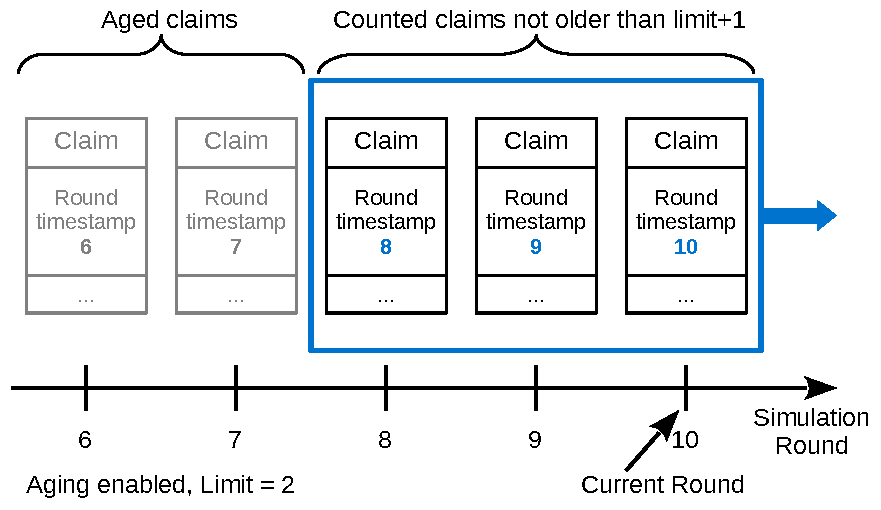
\includegraphics[width=0.85\linewidth]	{../images/improvement_aging-crop.pdf}
    \caption{
    Schematic showing the adaptation of aging as improvement technique.
    Aging maintains a window of time in which recent claims fall.
    These remain active and counted.
    Every claim older than the limit is removed.
    }
    \label{fig:improvement_aging}
  \end{center}
\end{figure}

\subsection{Aging}

Aging's purpose is to limit the memory of the reputation system, so as to help follow changes in agent behavior or sentiment.
Older data is forgotten, so no agent is locked into a reputation they no longer deserve.

Aging is adapted to the system as shown in fig.~\ref{fig:improvement_aging}.
\emph{Limit} specifies how long data is retained.
Any claim that is older than the limit is removed, along with all attached reviews.


\subsection{Weights}

\begin{figure}[tbp]
  \begin{center}
        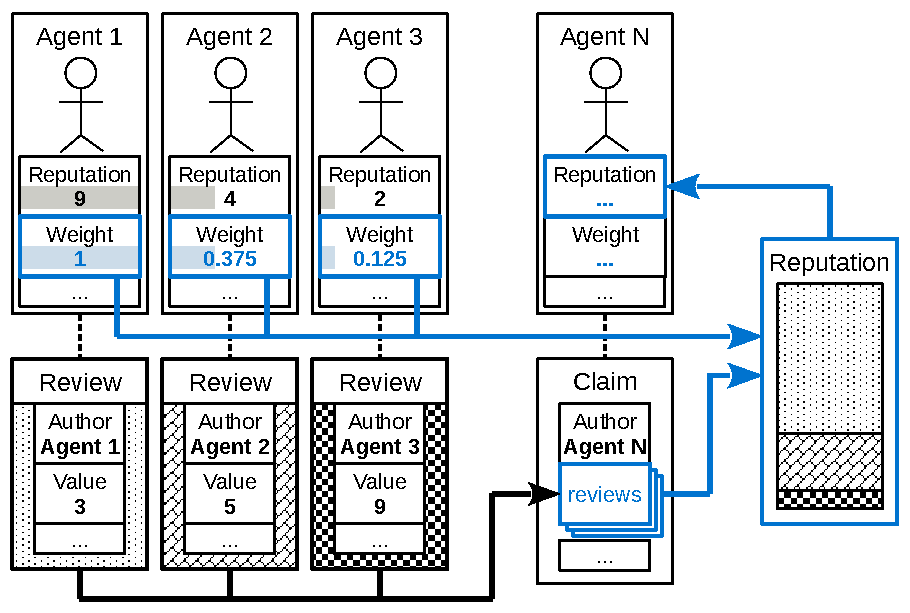
\includegraphics[width=0.85\linewidth]	{../images/improvement_weights-crop.pdf}
    \caption{
    Schematic showing the adaptation of weights as improvement technique.
    Whichever method is used to calculate \emph{Agent N}'s reputation, it also takes the weights of the raters into account.
    Their reviews are represented according to their weights.
    How agents get their weights can differ.
    Here, weights simply reflect the agent's reputation.
    }
    \label{fig:improvement_weights}
  \end{center}
\end{figure}

Weights aim to give preference to some agents over others when aggregating reviews.
The purpose of this is to give more weights to opinions of agents who have managed to build a good reputation, and less to those with bad reputation.
Intuitively, this acts in the opposite direction that aging, because weights preserve the status quo, while aging helps change it.

Figure~\ref{fig:improvement_weights} shows how weights are modeled.
An agent's reputation serves as its weights, calculated proportionally.
Reputation calculation methods use weighted average for aggregating reviews.


\subsection{Other Selected}

\emph{Outlier filtering} can be modeled by removing reviews which have significantly different valuations than the majority opinion.
This can be a way to prevent a small number of saboteurs to influence a claim's overall review valuation.
If the majority opinion of the claim shifts, the removed reviews need to be reconsidered and re-added if they are no longer outliers.

\emph{Anonymous ratings} serve to isolate the content from the content provider to prevent biased rating.
This is effectively implemented within the model if none of the agents use a strategy that discriminated against specific agents.

\emph{Rating range normalization} aims to even out different rating habits of agents.
For example, some agents avoid givin minimum and maximum ratings and stay at the middle ranges, others rate strong opinions more willingly.
Normalization extends the midrange rater's ratings to span the whole rating range.
This method is only applicable if agents already have a lot of ratings, because enough data is needed to confidently determine the typical rating range.


\subsection{Stakes}

Stakes is a new proposed improvement method.
It consists of claimers publishing a stake along new claims.
A stake gives how certain claimers are in their valuation of their new claim, i.e. the author's review.
A high stake signals confidence of the agent in the author review's accuracy, while a low stake notifies others that even the claimer is not sure whether its author review is correct.

Stake is a similar to a self reported weight, with a scope of only the involved claim.
Other agents and even reputation calculation can use the stake when making decisions.
For example, a low stake could mean the claimer does not receive much of a reputation penalty if the author review turns out to be inaccurate, while a higher stake incurs an amplified reputation correction.

Since stake requires providing an extra valuation with every claim, it is best suited for algorithmic systems.
A sensor can provide stakes based on its known uncertainty for example.



% --------------------------------------------------------------
\section{Distortion}\label{sec:distort_strategies}
% --------------------------------------------------------------
% other name: Attack Strategies

Distortion models the conscious and willing efforts of claimers to influence other's perception of their content quality.
It fits in the model as part of making new claims, seen in figure~\ref{fig:claim_rate_process}.
When an agent $A$ makes a new claim $C_A$, that agent has some valuation of what the claim's quality is.
This is called the measured quality $Q_{m,A,C_{A}}$ as per section~\ref{sec:approach_measure_claim}.
The claimer agent $A$ needs to make an author's review $R_{author A, C_{A}}$ about its new claim $C_A$.
Distortion basically defines how the agent comes up with the author review from the known the measured quality of the claim.
\begin{equation}
\mathrm{distort_{A}}(Q_{m,A,C_{A}}) = R_{author A, C_{A}}
\end{equation}

Distortion is one vector for agents to attack and exploit the reputation system, namely from the provider's side.
The most honest approach is to do no distortion at all.
Here, the author's review contains exactly the claimer's valuation of the claim quality.
Less honest agents can either state a higher or lower value than their own estimate.
To what extent and how often they do it depends on the distortion method they use.

%More complex distort schemes are the dynamic methods.



% --------------------------------------------------------------
\section{Rating}\label{sec:approach_rating_strategies}
% --------------------------------------------------------------

Rating models the feedback agents leave on content they used.
When an Agent $A$ rates a claim $C_B$ made by another agent $B$, a regular review $R_{A,C_{B}}$ is produced.

\begin{equation}
\mathrm{rate_{A}}(C_B) = R_{A, C_{B}}
\end{equation}

Rating is analogous to distortion in that both end up producing a kind of review.
The difference is that rating produces regular reviews on published claims, while distortion is used for author reviews.

Apart from this, rating may use a much larger amount of input data, everything that is part of or connected to the rated claim $C_B$.
This includes not only the measured quality, but also the other reviews of $C_B$, data of the author agent $B$ like $B$'s reputation, other claims of $B$ and their review and so on.
This allows modeling elaborate methods of feedback behavior.

Such amount of data is often not reasonable to utilize at once.
Therefore, models of rating usually select one valuation related to the claim, and then apply some manipulation to this value.
This input represents some numeric quality of the claim, like the author review, the quality as measured by the rater agent $A$, the average of other reviews, etc.
Comparing how well these perform can be a task of its own.
No specific value is assumed while discussing methods below.
The general notation $X$ is used instead.

Rating is the attack vector of those on the consumer side of transactions.
Many attacks and exploits found in related works can be modeled as rating methods, because reviews are usually the most important factor in calculating reputation.


\subsection{Simple Rate Methods}

Simple rating methods are characterized by using only one or a few input values and they can be described as a static transfer function.
The modeled ones are shown in figure~\ref{fig:simple_rate_strategies}.
Every transfer function can have parameters and an input $X$.

The two commonly considered attacked methods \emph{promotion} and \emph{slandering} can be modeled with linear or breakpointed linear methods, as in equations \ref{eq:rate_linear} and \ref{eq:rate_linear_brpoint}. Breakpointed can go both ways, setting a low or a high limit for a constant value before or after that respectively. Parameters: $a$, $b$, \emph{direction}, \emph{breakpoint} and \emph{breakpoint value}.
\begin{equation}\label{eq:rate_linear}
\mathrm{rate_{linear}}(C_B) = aX+b
\end{equation}
\begin{equation}\label{eq:rate_linear_brpoint}
\mathrm{rate_{breakpointed}}(C_B) = 
    \begin{cases}
      aX+b & \text{if $X$ within \emph{breakpoint}} \\
      \text{\emph{breakpoint value}} & \text{otherwise}\\
    \end{cases}
\end{equation}

Second order polinomial ratings described by (\ref{eq:rate_so}) are included from \cite{yu_detecting_2003}, where they are called exaggerated positive and negative.
Parameters: $a$, $b$, $c$ and \emph{direction}, the latter influencing if the polinomial is added or substracted.
\begin{equation}\label{eq:rate_so}
\mathrm{rate_{second order}}(C_B) = X \pm (aX^2+bX+c)
\end{equation}

Invert rating is also adapted from the above cited work.
\begin{equation}\label{eq:rate_invert}
\mathrm{rate_{invert}}(C_B) = -X + \mathrm{max}(X) + \mathrm{min}(X)
\end{equation}

Flattening was introduced to model the often-seen behavior of people avoiding strong opinions, tending toward the safe middle values.
It reduces the more extreme values towards the middle range.
The strength of flattening is given by parameter $a < 1$.

\begin{equation}\label{eq:rate_flatten}
\begin{aligned}
&\mathrm{rate_{flatten}}(C_B) = a(X-mid)+mid \\
\mathrm{where~}&mid = 0.5\big(\mathrm{max}(X) - \mathrm{min}(X) \big) + \mathrm{min}(X)
\end{aligned}
\end{equation}

Flattening can be seen as conservative rating.
The opposite of flattening is when the transfer function amplifies toward extremes.
Flatten rating in (\ref{eq:rate_flatten}) can do this with a multiplier $a > 1$.
This can be a model for agents that mostly have strong opinions, either very high or very low.

Finally, the simplest of all rating methods is when nothing is done.
This means some quality $X$ of the claim is returned without altering.
An example is the method that simply repeated the author's review of the rated claim.

\begin{figure}[tbp]
  \begin{center}
    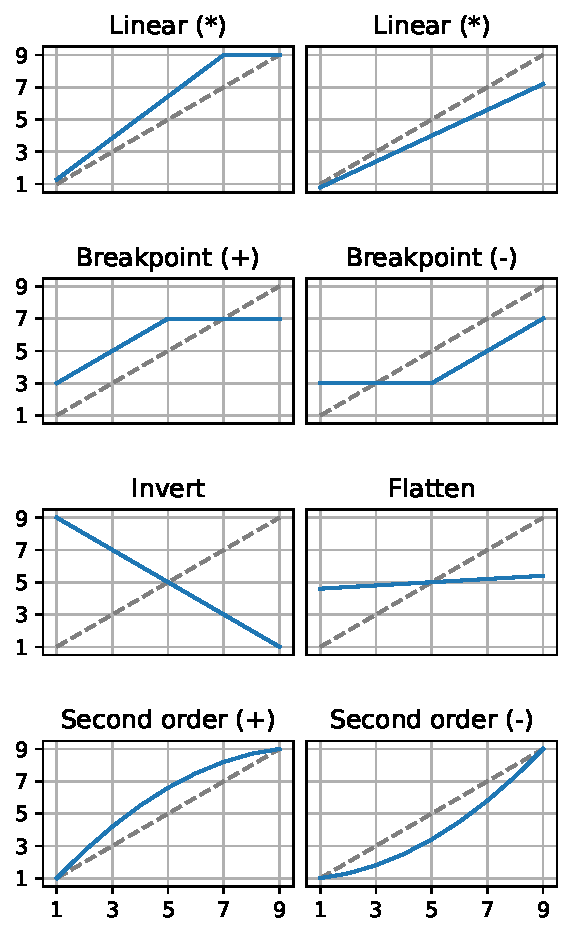
\includegraphics[width=0.74\linewidth]{../images/simple_rate_strategies2.pdf}
    \caption{
    Transfer functions of simple rating methods.
    The dashed line is the input without transformation.
    It can be any single value from the rated claim, for example its author review, or measured quality.
    Rating methods show example parametrizations, these can of course change.
    Both the input and ratings are selected to be within $[1,9]$.
    }
    \label{fig:simple_rate_strategies}
  \end{center}
\end{figure}


\subsection{Random Rate Methods}
Random error rating is a method where sometimes a significantly inaccurate rating is made.
	It can model a sensor's rare erroneous data.
Also, agents whose attack approach is rate normal most of the time to build reputation and occasionally insert a malicious rating.
The malicious rating may carry more weight due to the rater's otherwise good reputation.
The method is modeled as per (\ref{eq:rate_random_error}).
Parameters: \emph{chance}.
\begin{equation}\label{eq:rate_random_error}
\mathrm{rate_{random~error}}(C_B) = 
\begin{cases}
random & \text{if $chance$ is taken by coincidence} \\
X & \text{otherwise}
\end{cases}
\end{equation}

Various other random ratings can be used to model actors who want to weak havoc or are completely ignorant.
Random, lower half, and higher half random all give a random value within the whole or part of the rating range.
\begin{equation}\label{eq:rate_random}
\mathrm{rate_{random}}(C_B) = \text{random value in $\big[\mathrm{min}(X), \mathrm{max}(X)\big]$}
\end{equation}
\begin{equation}\label{eq:rate_random_higher_half}
\mathrm{rate_{random~higher~half}}(C_B) = \text{random value in $\left[\frac{\mathrm{min}(X)}{2}, \mathrm{max}(X)\right]$}
\end{equation}
\begin{equation}\label{eq:rate_random_lower_half}
\mathrm{rate_{random~lower~half}}(C_B) = \text{random value in $\left[\mathrm{min}(X), \frac{\mathrm{max}(X)}{2}\right]$}
\end{equation}


\subsection{Rate Methods of Collectives}
Collaborating agents working towards a common goal can form collectives.
Such groups are common in real online reputation systems.
Producers often have a loyal following among consumers, who will promote the producer's content with higher ratings.
Some marketing or other agencies take clients to improve their online reputation by a coordinated promotion attack.
Producers might also initiate slandering-type attacks against competitors.
This is sometimes done by organized or spontaneous mobs, leaving baseless bad reviews on businesses or sellers for various reasons.

A main distinction is whether the collective promotes or slanders.
Slandering is typically aimed towards an agent outside the collective.
Promotion on the other hand can target members of the collective.
As also mentioned before, a collective can build up the reputation of its members by promoting each other, so that a later planned slander attack carrier more weight.

\subsection{Experience-Based Rate Methods}
Experience-based rating is when a consumer judges a content based on personal experience with it.
An agent's own experience is modeled by measuring claims, discussed in section~\ref{sec:approach_measure_claim}.
When an agent $A$ measures the claim $C_B$ made by agent $B$, it results in the measured quality $Q_{m,A,C_{B}}$.

Technically any of the discussed rate methods can be experience-based, if $X$ is chosen as $Q_{m,A,C_{B}}$.
Still, explicitly defining such a rate method is worth it because rating from own opinion is common.
\begin{equation}\label{eq:rate_own_experience}
\mathrm{rate_{own~experience}}(C_B) = Q_{m,A,C_{B}}
\end{equation}



% --------------------------------------------------------------
\section{Evaluation}\label{sec:approach_evaluation_framework}
% --------------------------------------------------------------
% aka. Simulation System
% putting together all the above

%check how to implement these
%can use existing eval frameworks? or need own one in python
%if latter, what components
%a diagram can be good also for the presentation

There have been many reputation evaluation frameworks made in the past, as surveyed in chapter~\ref{chap:related_work}.
The first approach was to find one of these suitable for use, for which a few general requirements were applied.
These are:
\begin{itemize}
    \item available source code
    \item domain-independence
    \item preferrably widely accepted
    \item extendability and ease of modification
    \item flexibility with simulation parameters and components
    \item preferrably some common reputation schemes already implemented
\end{itemize}

Most of these are needed to accomodate unique approaches and fulfill specific requirements, such as:
\begin{itemize}
    \item the use of one or more reputation improvement methods
	\item ability to implement custom reputation schemes
    \item flexible review values (custom integer ranges)
    \item second-order rating schemes (like stakes)
    \item ability to represent \glspl{claim} in some form
    \item can define custom evaluation metrics
    \item full simulation of all agents
\end{itemize}

None of the examined evaluation frameworks satisfied all needs.
Overall requirements and unique approaches warranted the inception of a new reputation simulation framework.

Because of this, a custom system was designed to simulate, compare and evaluate selected reputation schemes under various environmental conditions.
This section gives a conceptual introduction, including components and core features.
For a description of the concrete Python implementation, see Chapter~\ref{chap:implementation}.



\subsection{Scenarios}\label{sec:scenario}
A \gls{scenario} is the description of a complete reputation environment including the reputation schemes and agents with various behaviors.
All parameters that are needed during simulation are part of the scenario.
Some of the most important are:
\begin{itemize}
	\item how reputation values are calculated
	\item which reputation improvement methods are applied
	\item the size of the agent population
	\item how agents behave during simulation
	\item how long the simulation goes (i.e. how many rounds)
	\item the possible rating and reputation values (e.g. binary, integers 1 to 5)
	\item what seed is used to generate random numbers
	\item what graph and data exports metrics should be created
\end{itemize}

In this way, a scenario encapsulates all that is in a single simulation.
This helps organize combinations of simulation parameters, and compare them.
For example, when the goal is to see what effect malicious agents have, one could draft separate scenarios with varying percentage of malicious agents ranging from 0\% to 100\% in each.


\subsection{Measuring Claims}\label{sec:approach_measure_claim}
Measuring claims is the term used for when an agent assesses the quality of a claim.
This models when a consumer upon receiving a content, tries it out and leaves feedback based on first-hand experience.
Additionally, an agent can also measure its own claim.
%Measuring a claim is the representation of trying out a product or content and making an opinion of what its quality could be.

The measured quality $Q_{m,A,C_{B}}$ denotes agent $A$'s assessment of claim $C_B$.
With the model's assumption on the existence of a ground truth, measuring a claim can be seen as an agent trying to guess this hidden quality valuation.
Agents are modeled here with various levels of expertise, which affects how close or how reliably they can measure the ground truth.
Know-how, experience, expertise or inside knowledge are among the possible factors playing a role.
This can vary between implementations.
Pyrepsys uses \acrlong{ctai} for this.
It is a parameter of agents representing the maximum inaccuracy they can make when measuring.

As discussed in section~\ref{sec:appr_claim_rate_process}, making a new claim has two main stages: measuring the ground truth and distorting.
The measurement serves as input for distortion.
Distortion models conscious actions, honesty or willing manipulation.
Measuring claims is also a sort of distortion, albeit not under the control of the agent.
While distortion is \emph{intent}, measurment represents \emph{competence}.


\subsection{Claiming and Rating}\label{sec:appr_claim_rate_process}
Claiming (figure~\ref{fig:claim_rate_process}, above) spawns a new claim $C_A$ without any reviews, containing a \gls{gr_truth}.
The claimer agent $A$ measures this hidden quality and distorts it, resulting in a value representing the clamer's opinion of his own claim.
This is attached as an \gls{author_review} $R_{authorA,C_{A}}$ to the claim to be published.

Rating (figure~\ref{fig:claim_rate_process}, below) takes an existing published claim $C_A$ by agent $A$.
The rater agent $B$ takes all data relevant to claim $C_A$ and produces a \gls{review} $R_{B,C_{A}}$.
This is then appended to the other reviews on claim $C_A$.

\begin{figure}[tbp]
  \begin{center}
        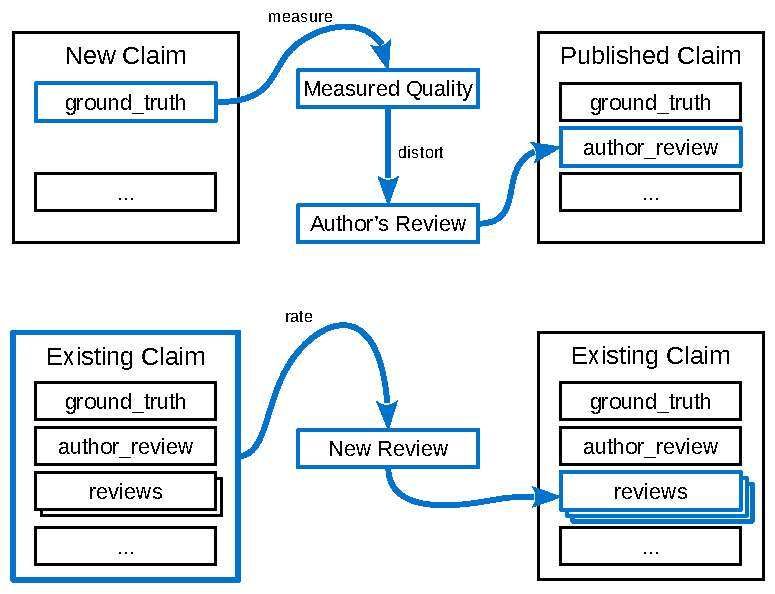
\includegraphics[width=1\linewidth]	{../images/claim_rate_process-crop.pdf}
    \caption{
    Schematic representation of claiming (above) and rating (below) processes, with the involved claims and reviews.
    }
    \label{fig:claim_rate_process}
  \end{center}
\end{figure}



\subsection{Resolution}\label{sec:approach_resolution}
Resolution determines what values are allowed in various parts of the model.
For example, if reviews are constrained by a resolution of 1, and minimum and maximum values are 1 and 9, then the result of ratings can be integers from 1 to 9, i.e. $\forall R$: $R\in\mathbb{Z}$ and $1 \le R \le 9$.

There are two main uses for resolution.
One of them is the already mentioned review resolution.
It applies to any review made, and its purpose is to force review values to follow the wished reputation scheme.
With separate resolution handling, rate and distort schemes remain independent of the exact selection of allowed values they are expected to produce.
This means they do not need to be customized along this, their results will simply be changed to the nearest resolution step.

The other use is with measured claim quality values.
Measured claim resolution effectively limits how finely grained agents can assess claim ground truths.
For example, let review resolution be 1 and measurement resolution be 0.5.
Here, reviews are strictly integers.
But when agents assess a claim's quality by measurement, they may get a value between two integers too.
For example, a measurement of 2.5 signifies the agent thinks the claim is better than 2 and worse than 3.
The agent will still not be able to publish a review of 2.5 because the review resolution is 1.
However, the information is there, what the agent does with it is left for the agent to decide.

The idea behind limiting measured claims in this way is the following.
When thinking of what quality a content (claim) has, it is often not possible to exactly determine it.
For example, in the 5-star scheme, one could think something is around 3 or 4 out of 5, but not give a more exact estimate.
Measuring claims models this thought process.
If measurement would give 3.4562 in this case, there is no uncertainty where exactly the quality falls.
If resolution is at 0.5, measurement can only return either 3, 3.5 or 4, or even other values if the agent has a huge inaccuracy.
A similar but slightly better claim would also measure at the same values.
This is more realistic when agents represent people judging content freely.
On the other hand, a more fine-grained resolution could be used when the scenario works with an algorithmic reputation environment.
Where agents are machines and there is a way to algorithmically assess a claim, it is reasonable to allow more freedom for claim measurements.

A third resolution domain could also be created for reputations, limiting the granularity of global reputations.
The reason this was not included is that reputation calculation methods serve as a single source of reputation values.
They can adhere to specific resolution limits as part of their calculation if needed.
For example, if a reputation strategy is build to rate in the 5-star system, it is implemented to give integers [1,5] anyway.
On the other side, a scenario can have many different kind of behaviors for agents.
Designing multiple versions of each with different resolutions unreasonable, hence the review resolution domain.




% CHAPTER ######################################################################
\chapter{Implementation}\label{chap:implementation}
% ##############################################################################
%Implementation: If you did one, explain all the details here: hardware (chips, buses), OS, compiler, libraries, data structures and their field sizes.

\lettrine{S}{imulations} are done with a custom-made python simulation framework named Pyrepsys.
This chapter gives the implementation-specific details of Pyrepsys. 
For a conceptual description, see Section~\ref{sec:approach_evaluation_framework}.

Pyrepsys is a one-stop solution for simulating, comparing and evaluating reputation schemes.
Simulation of scenarios is performed on a round-by-round basis.
Shared configuration among scenarios, simulating batches of scenarios in succession and controlled random number generation help compare different scenarios.
Evaluation is aided by metrics.
They are data processors that automatically generate graphs and export data from simulations.

Flexibility and extendability are among the main design objectives of Pyrepsys.
Variables can be altered in scenario configuration files.
The size and composition of the agent population is customizable.
New agent behaviors, metrics, reputation calculation and improvement methods can be easily added.

Miscellaneous supportive functionalities are also discussed in this chapter.
A scenario configuration creator can be used to make a batch of scenarios with variations along selected configuration parameters.
Extensive automated self-testing can verify the integrity of the simulation framework if any changes are made.
Finally, profiling and benchmarking tests are provided to identify simulation bottlenecks and measure performance.

Additional references for using Pyrepsys are provided outside this chapter.
For a description of the Pyrepsys command-line interface, refer to Appendix~\ref{appendix:cli_invocation}.
A complete list and explanation of possible scenario configuration parameters are found in Appendix~\ref{appendix:scenarios}.
% Finally, information regarding the scenario creator 

% TODO: prerequisites, dependencies, tested versions, environment
% TODO: reference table~\ref{tab:pyrepsys_modules}
% TODO: also describe concrete implementations of behavior and reputation strategies, improvement handlers ?

\begin{table}[tbp]
\centering
\begin{tabular}{@{}lll@{}}
\toprule
\textbf{Module} & \textbf{Notable Classes} & \textbf{Responsibility}    \\ \midrule
agent               & \emph{Agent}, \emph{Claim}, \emph{Review} &Define agents with the simulation data structure \\
behavior            &  &Submodule. Define agent rate and distort strategies \\
config              & \emph{Configurator} &Scenario configuration related. Read, parse, provide configs. Prepare other classes. \\
errors              &  &Custom exceptions \\
helper\_types        & \emph{SimulationEvent}, \emph{ResolutionDomain}, \emph{LocalConfig}& Accessory type definitions \\
helpers             &  &Accessory function definitions. Resolution handling, Internal-Agent-Exposed conversion \\
instantiator        & \emph{Instantiator} & Creation of metric, reputation strategy, behavior strategy and improvement handler instances \\
main                &  &Program entry point, preparation of logging and directories, coordination of simulation \\
metrics             &  &Submodule. Defines data export and graph drawer metrics \\
paths               &  &Directory paths \\
reputation          &  &Submodule. Define improvement handler and reputation strategy classes \\
results\_processor   & \emph{ResultsProcessor} &Containment and coordination of metrics \\
scenario\_creator    &  &scenario creator utility \\
scenario\_simulator  & \emph{ScenarioSimulator} &Simulate one single scenario. Aka System \\
\bottomrule
\end{tabular}
\caption{
	Modules making up Pyrepsys.
	Modules \texttt{behavior}, \texttt{reputation} and \texttt{metrics} form submodules.
	TODO FIX THE TABLE PARTS ARE OUT OF THE WORLD
}
\label{tab:pyrepsys_modules}
\end{table}

% --------------------------------------------------------------
\section{Simulation Flow}\label{sec:impl_simulation}
% --------------------------------------------------------------

Simulation in Pyrepsys is built around \glspl{scenario}.
Each invocation consists of simulating one or more scenarios after each other.
At the beginning, the default scenario configuration is fetched.
Then Pyrepsys reads and applies the individual configuration for each scenario.
The scenario is simulated after these preparations.
Conducting the simulation is the responsibility of the \emph{ScenarioSimulator} class.
Once all scenarios are finished, the results processor module exports collected data and draws graphs based on the selected metrics.
The simulation part's schematic flow is shown in figure~\ref{fig:simulation_flow}.

Scenario simulation is performed on a round basis.
The number of rounds is part of the scenario configuration.
Each round consists of four distinct phases:

\begin{enumerate}
	\item claiming
	\item rating new claims
	\item applying reputation improvements
	\item reputation calculation
\end{enumerate}

\subsection{Claiming}
Claiming is the part where agents can make new \glspl{claim}.
During this phase, all agents get an opportunity to make one new claim.
Whether an agent ends up publishing a claim or not depends on multiple factors.

First of these is the agent's \gls{claim_probability}.
This represents the likelihood of them attempting a claim if given an opportunity.
A more consumer-type agent would have a lower probability and thus claim rarely if ever.
On the other hand, producer-type agents would tend toward higher probabilities, and claim more often.
The random check whether agents attempt a claim or not is performed on the \gls{main_rng_chain}.

If the agent passes this check, a claiming process begins.
First, a claim is generated containing a random \gls{gr_truth}. 
The ground truth is not directly accessible for the agent.
It can however be measured, which is the second step of the claiming process.
Measurement results in the \gls{measured_claim_score}, which represents an approximation of the claim's true quality.
How good this approximation is, depends on the agent's ability to assess claims.
Further details of measuring claims is described in section~\ref{sec:approach_measure_claim}.

With the measured truth, the agent executes its \gls{distort_strategy}.
It essentially applies one of the distortion methods found in section~\ref{sec:distort_strategies}.
The resulting value is the \gls{distorted_claim_quality}.

At this point the agent checks whether the distorted quality falls in the agent's \gls{claim_range}.
Claim range serves as a minimum and maximum limit as to what claims an agent is willing to publish.
If the distorted claim quality falls outside these limits, the claim is discarded and claiming is aborted.
In this case, the agent will not claim in this round.

If the limits are not violated, the agent prepares the claim for publishing.
The \gls{author_review} is created and appended to the claim.
Its value is always the distorted claim quality from the previous step.
Finally, the agent appends the claim to the list of his claims, and so the claim is published.
The claiming process is illustrated on figure~\ref{fig:claim_rate_process}.

\begin{figure}[tbp]
  \begin{center}
        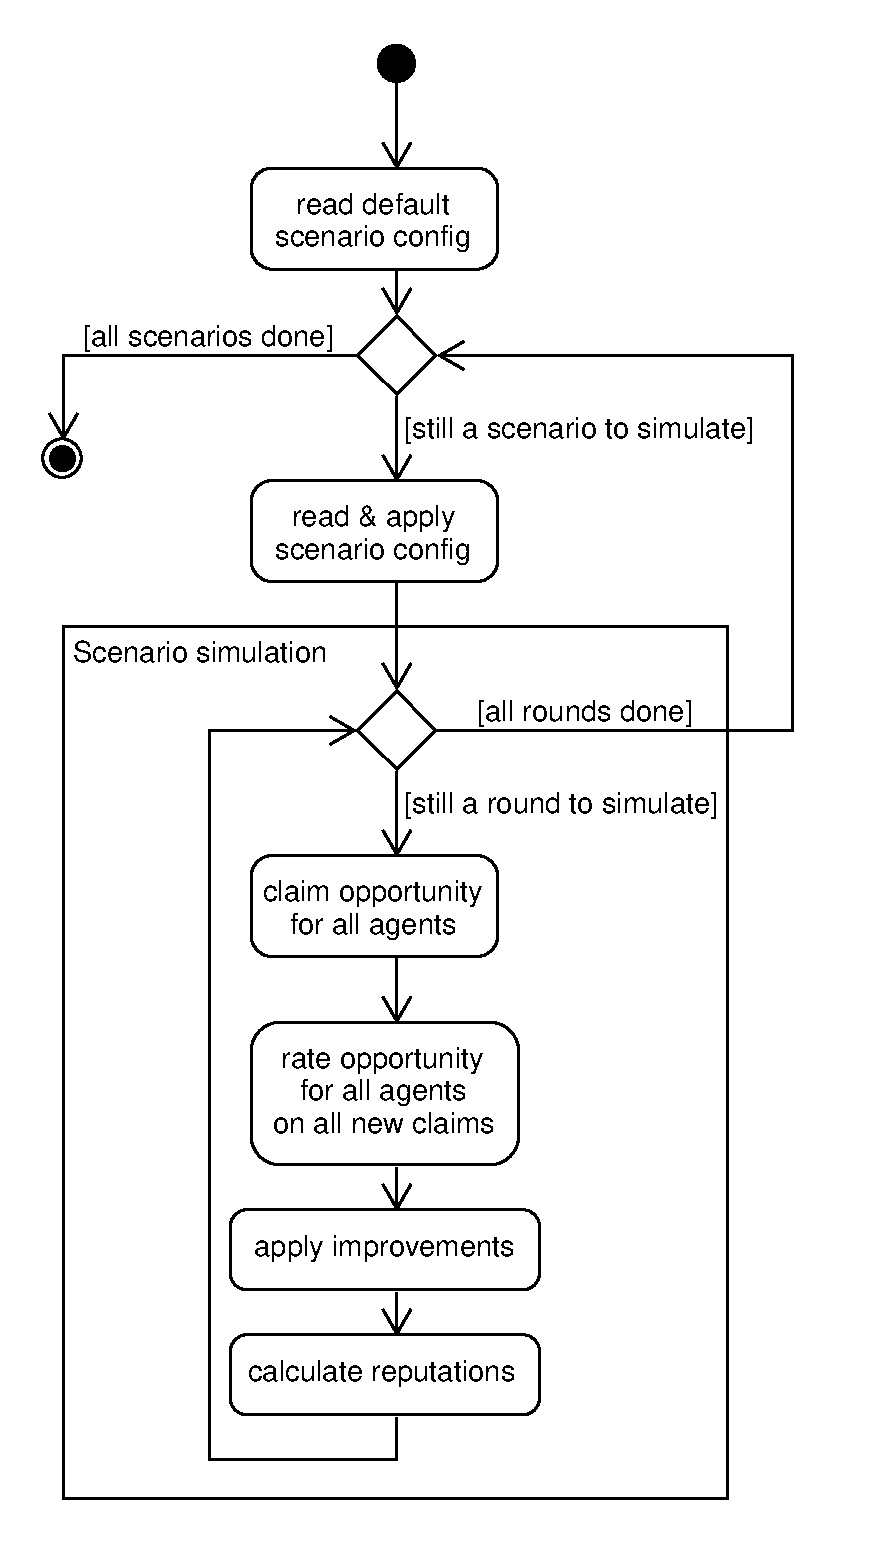
\includegraphics[width=0.75\linewidth]	{../uml/simulation_flow.pdf}
    \caption{
    Simulation flow in Pyrepsys.
    A single simulation unit is the \gls{scenario}.
    Each \gls{scenario} is simulated independently after one another.
    Rounds make up the simulation within a \gls{scenario}.
    Each round consists of four distinct phases: claiming, rating, improvement and reputation calculation.
    The number of rounds is specified in the configuration.
    }
    \label{fig:simulation_flow}
  \end{center}
\end{figure}


\subsection{Rating}

Rating stage is when agents can rate claims published in the current round.
Each new claim made in the previous section is put up for rating.
For each of these claims, every agent other than the claimer is given an opportunity to rate it.
The maximum possible number of \glspl{review} made during one round is show in equation~\ref{eq:max_reviews}.

\begin{equation}\label{eq:max_reviews}
	\mathrm{max}(N^r_{reviews}) = N^r_{claims} (N_{agents}-1)
\end{equation}
Where $ N^r_{claims} $ and $ N^r_{reviews} $ are the number of claims and reviews made in the current round $r$.
$ N_{agents} $ is the number of agents in the current scenario.

Similarly to claiming, agents are given opportunities to rate a claim.
Whether or not they take it and leave a review depends on the agent's \gls{rate_probability}.
This percent chance represents each agent's willingness to rate encountered claims.
A low rating probability means the agent is passive and rates seldom.
A higher chance to rate represents an enthusiastic agent that often makes reviews of claims.
Each time an agent is given a chance to rate, a check is performed on the \gls{main_rng_chain}.

If this check is passed, the agent makes a review.
The schematic process of rating is shown on figure~\ref{fig:claim_rate_process}.
It consists of executing the agent's \gls{rate_strategy} with the claim under review as input.
This is done to enable a wide range of rating methods.
The claim's other reviews, the author's review, the author's identity or the rater's own measurement of the claim \gls{gr_truth} may all play a role in determining the review value.

Once the review value is ready, a review object is created.
It is appended to the review list on the claim and also to the rater agent's list of own reviews.
With this, the review is published and the agent has finished the claiming process.
The same agent can possibly make a review in the same round again, but only when rating another claim.


\subsection{Applying Improvements}

Improvements are the third main step of rounds.
At this phase, all claims and reviews of the current round have been published.
These were added to their appropriate places into the data structure formed by the list of agents.
As discussed in detail in section~\ref{sec:impl_data}, it contains all simulation data from the current scenario.
This is passed to the selected improvement methods by the \emph{ScenarioSimulator} for processing.
All modifications are done on this mutable list of agents.

Improvement methods are implemented as separate handler classes.
These handlers form a handler chain as per the \emph{chain of responsibility} software design pattern.
See figure~\ref{fig:improvement_handlers} for an UML model.
Each handler is formed by inheriting from \emph{reputation::AbstractHandler}.
This abstract class defines the interface improvement handlers need to adhere to.
It also gives the default behavior for the handlers.
The method \texttt{handle(request)} is the default behavior of calling the next handler in the chain if any, or simply returning if the current handler is the last in the chain.
This behavior is meant to be executed at the end of all concrete improvement subclass \texttt{handle()} calls like this: \lstinline{return super().handle(agents)}.
\emph{AbstractHandler}'s second method \texttt{set\_next(handler)} is used to build the handler chain by giving which handler comes after this one is finished.
Normally this is done by the configuration module during scenario preparation.

Organizing the improvements as a handler chain has multiple benefits.
Firstly, improvements remain modular and flexible.
Separate handlers can be added to or removed from simulations.
The order of handling is free to change.
Implementing new improvements is easily done by inheriting from the abstract handler class.
Furthermore, the client code calling the handlers does not depend on which handlers are active.
This means \emph{ScenarioSimulator} is independent of improvements.
Apart from a simple structure, this allows changing the order or composition of the chain during runtime.
Although this is not currently supported, implementing this feature is simple.
Finally, by putting improvement methods in a class, they are encapsulated.
As such, there is a clear distinction between data and methods related to improvements and other parts of the system.

\begin{figure}[tbp]
  \begin{center}
        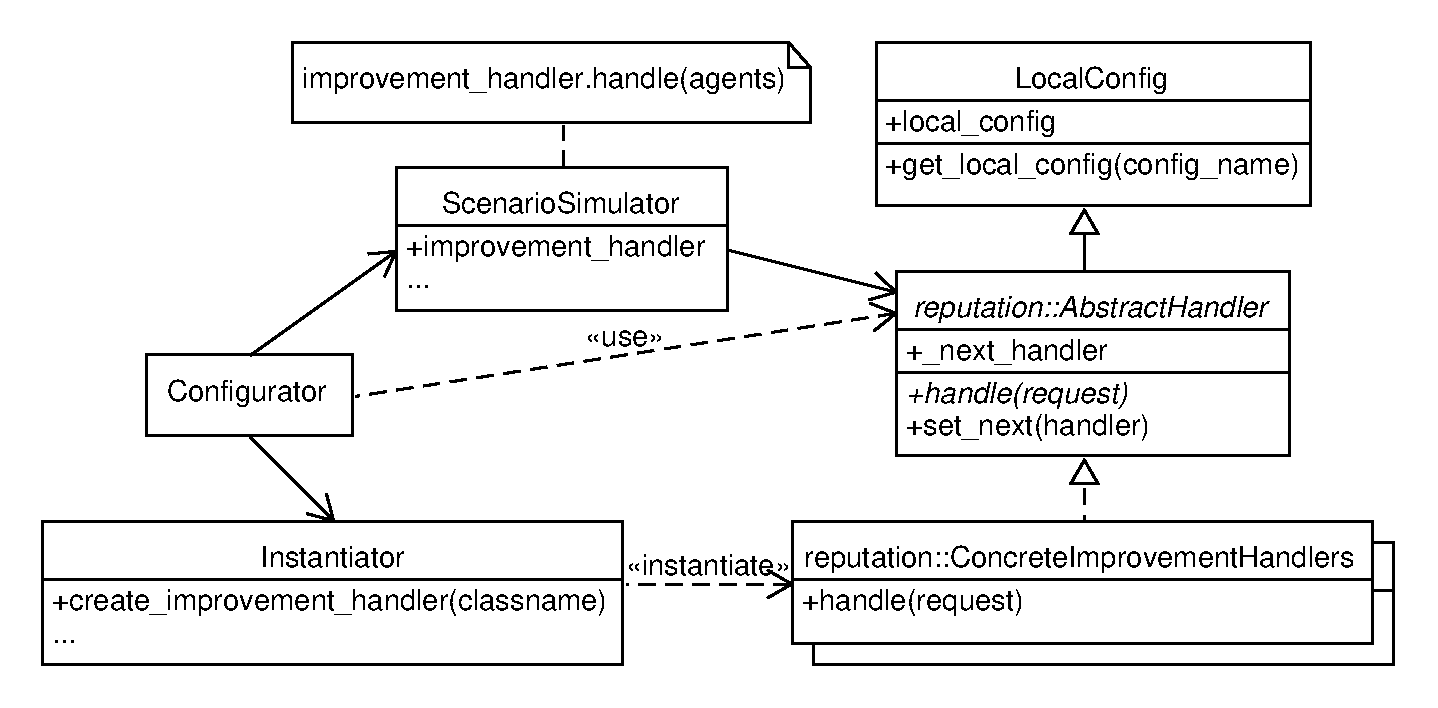
\includegraphics[width=1\linewidth]	{../uml/improvement_handlers.pdf}
    \caption{
	UML class diagram of improvement handlers. 
	\emph{Configurator} creates instances of the required improvement handlers via the \emph{Instantiator} and sets the handler chain's entry point in \emph{ScenarioSimulator}.
	When improvements are due, \emph{ScenarioSimulator} calls the first handler with the agents data, which includes all claims and reviews.
	\emph{LocalConfig} provides custom configuration for each individual improvement handler.
	This is discussed in section~\ref{sec:local_config} in detail.
    }
    \label{fig:improvement_handlers}
  \end{center}
\end{figure}

\subsection{Reputation Calculation}\label{sec:impl_reputation_calculation}

After improvements have finished, the fourth and final step of a simulation round is calculating agent reputations.
Reputation calculation methods are implemented with the strategy software design pattern.
Each reputation scheme is implemented as a class that inherits from a common abstract parent class, \emph{reputation::ReputationStrategy}.
This class provides a simple interface containing the method \texttt{calculate\_reputations(agents)} which concrete strategies must implement.

After improvements have finished, \emph{ScenarioSimulator} starts reputation calculation by calling this method on the reputation strategy it stores.
The method takes the mutable list of all agents of the scenario as input.
Then the reputation strategy's single responsibility is calculating agent reputations based on whatever method it employs and updating each agent's \texttt{global\_reputation} attribute with it.
This holds the agent's latest public reputation score.
Before the first reputation calculation takes place, it holds an initial reputation set according to configuration before the first round.

Using the strategy pattern allows modularity and flexibility, much of the same advantages with improvement handlers.
New reputation strategies are easy to add to Pyrepsys by creating a subclass of \emph{reputation::ReputationStrategy} in the \texttt{reputation} subpackage and putting the classname on the import list.
Strategies are independent of the client class, \emph{ScenarioSimulator}.
This means they are simple to exchange.

Additionally, encapsulating reputation schemes into classes makes them self-contained and forms a clear structure.
Figure~\ref{fig:reputation_strategy} shows the UML model of reputation strategies.
implemented with the strategy pattern

\begin{figure}[tbp]
  \begin{center}
        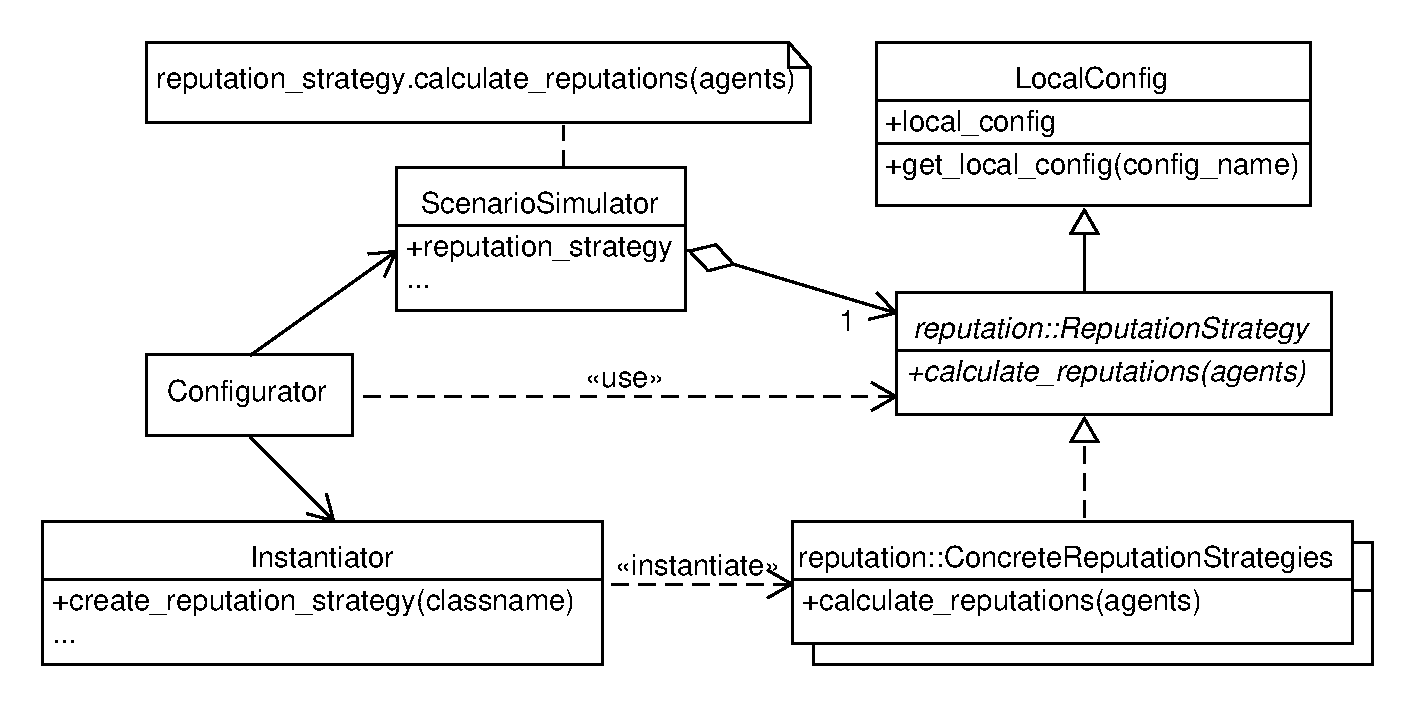
\includegraphics[width=1\linewidth]	{../uml/reputation_strategy.pdf}
    \caption{
	UML class diagram of reputation strategies.
	\emph{Configurator} creates an instance of the selected reputation strategy via the \emph{Instantiator} and gives it to \emph{ScenarioSimulator}.
	At reputation calculation, \emph{ScenarioSimulator} calls its reputation strategy object with the agents data, which includes all claims and reviews.
	\emph{LocalConfig} provides custom configuration for strategy instances.
	This is discussed in section~\ref{sec:local_config} in detail.
    }
    \label{fig:reputation_strategy}
  \end{center}
\end{figure}



% --------------------------------------------------------------
\section{Agents}\label{sec:impl_agent}
% --------------------------------------------------------------

\subsection{Behavior Strategies}
Behavior strategies serve as the implementation of agent's rating or distortion methods.
The \emph{behavior} subpackage contains related classes.
Both rating and distortion strategies are implemented very similarly to reputation strategies as described in section~\ref{sec:impl_reputation_calculation}.

The involved classes are shown in the UML diagram in figure~\ref{fig:behavior_strategies}.
Both behavior strategy types share a common abstract ancestor called \emph{BehaviorStrategy}.
This class serves two main purposes.
First, it describes a common interface for both rate and distort strategies.
This consists of the \lstinline{execute()} function, which takes as parameter the calling agent, some data that is needed for the rating or distortion method, and an optional random seed.
Second, the common ancestor provides shared functionality for random number generation with the \lstinline{rng()} method.
This can be used by behaviors to start a \gls{branchoff_rng_chain} and generate random numbers.

Distortion and rating diverge with their own abstract adapter classes \emph{DistortStrategy} and \emph{RateStrategy}.
Both are child classes of the common ancestor class.
Their main purpose is to enable the same random chain functionality while also providing a different interface for both behavior types.
\emph{DistortStrategy} provides \texttt{distort()}, \emph{RateStrategy} provides \texttt{rate\_claim()}.
Both classes wrap \texttt{execute()} calls to their respective behavior calls.
Additionally, the adapter makes a preemptive check on the input data.
\emph{RateStrategy} allows \emph{Claim} objects to be passed, while \emph{DistortStrategy} allows \gls{measured_claim_score} values: integer and float.

Finally, concrete strategies of both types derive from the abstract adapter parents.
\emph{Configurator} creates the concrete behavior strategy instances via \emph{Instantiator} and assigns them to each agent according to scenario settings.
Agents then call upon their behavior strategies during simulation through the \texttt{execute()} interface.

\begin{figure}[tbp]
  \begin{center}
        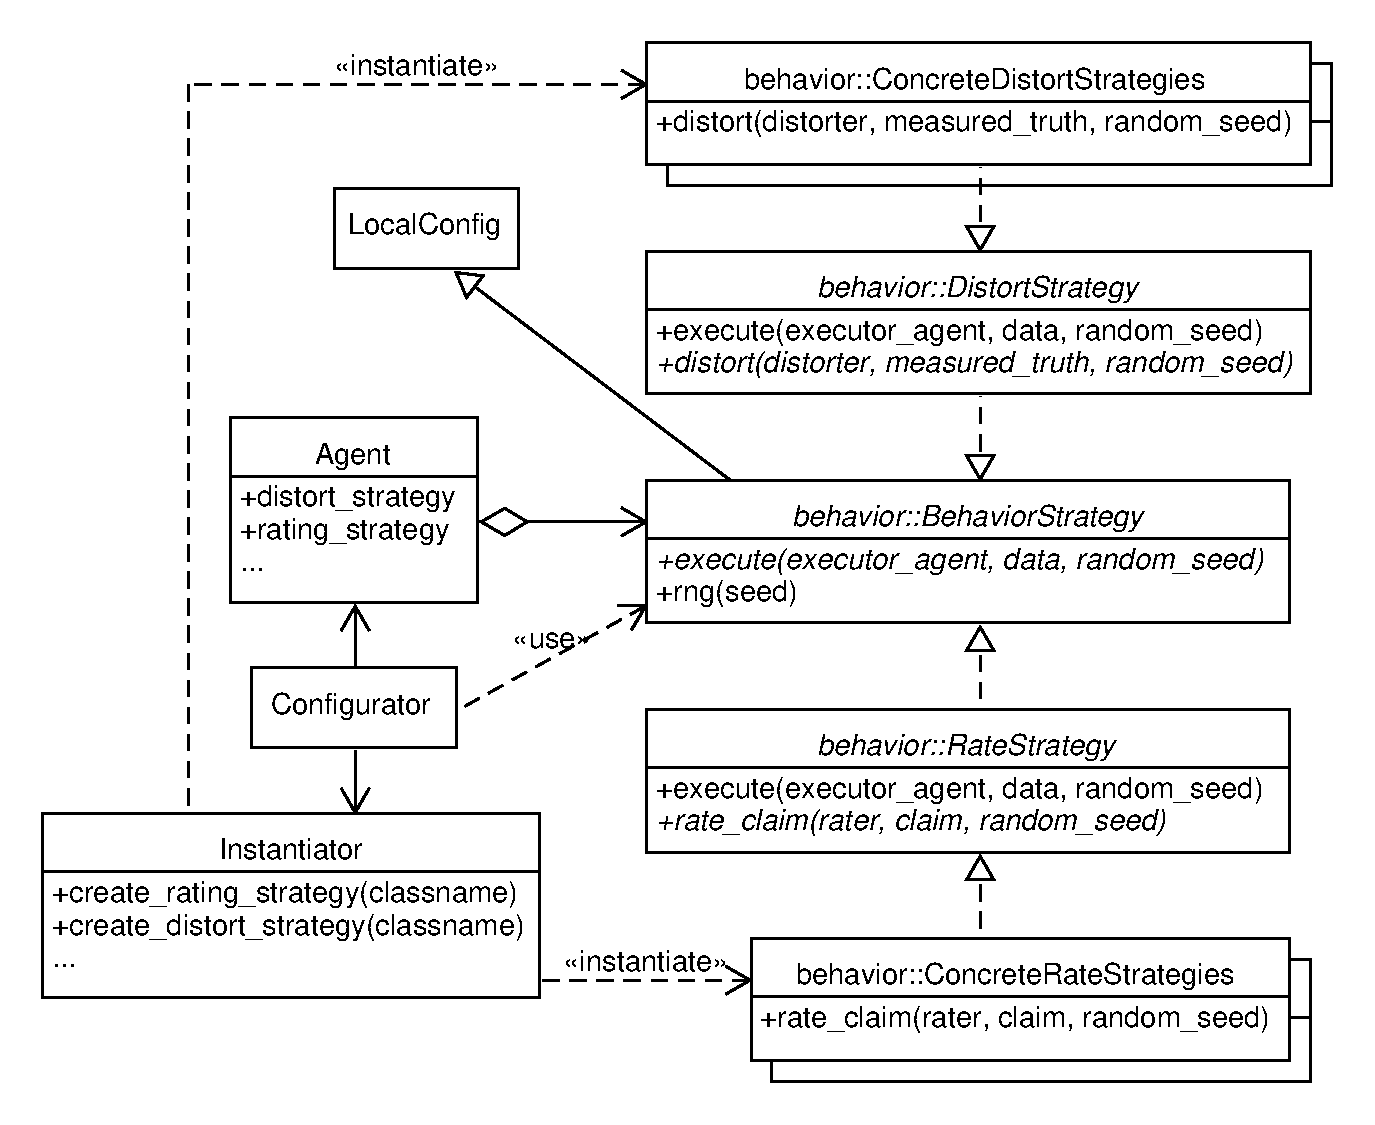
\includegraphics[width=1\linewidth]	{../uml/behavior_strategies.pdf}
    \caption{
	UML class diagram of agent behavior strategies.
	The abstract class \emph{behavior::BehaviorStrategy} serves as a common base for both distort and rate strategies.
	Two interface classes \emph{behavior::RateStrategy} and \emph{behavior::DistortStrategy} both inherit from it.
	Concrete strategies are descendants of these two classes.
	\emph{Configurator} creates behavior concrete strategy instances via the \emph{Instantiator} and sets them on the agent using it.
	When rating or distorting, the agent calls \lstinline{execute()} on the appropriate behavior strategy.
	\emph{LocalConfig} provides custom configuration for strategy instances, discussed in section~\ref{sec:local_config} in detail.
    }
    \label{fig:behavior_strategies}
  \end{center}
\end{figure}


\subsection{Measuring Claims}
Measuring is taking an approximation on the hidden true quality, or the \gls{gr_truth} of a claim.
It results in a value that is comparable to the ground truth or any review on the claim.
This is the \gls{measured_claim_score}.

Since assessing the quality of a claim depends on the assessing agent's know-how, experience or expertise, this is reflected in claim measurement as well.
Agents have the attribute called \gls{ctai} for this.
This represents the accuracy the agents can guess a claim's ground truth.
\Gls{ctai} is given for each agent in the scenario configuration.
The value of \gls{ctai} is the maximum error an agent can make when assessing a ground truth in each direction.
This is represented in equation~\ref{eq:ctai}.

\begin{equation}\label{eq:ctai}
C_{gr~truth} - \mathrm{\acrshort{ctai}} <= \mathrm{measured~quality} <= C_{gr~truth} + \mathrm{\acrshort{ctai}}
\end{equation}

Whenever an agent needs to measure a claim, it calls its method \lstinline{measure_claim()}
This takes as argument the claim to be measured and a random number generator.
Since claims are measured on-demand, the generator is always a \gls{branchoff_rng_chain}.
The measurement error is created as a random value with uniform distribution between [-\acrshort{ctai},~\acrshort{ctai}].
This is then added to the claim's true quality.

\begin{equation}\label{eq:measure_claim1}
\mathrm{measurement~error = rng.uniform(-\acrshort{ctai}, \acrshort{ctai})}
\end{equation}
\begin{equation}\label{eq:measure_claim2}
\mathrm{measured~quality} = C_{gr~truth} + \mathrm{measurement~error}
\end{equation}

The above equations summarize how claim measurements are made.
Theoretically, an agent could find out the true quality of a claim by making multiple measurements.
This is prevented by doing measurements inside the \emph{Agent} class before any other parts of the code are called where the measured quality is needed.
Currently only one such case exists.
Measured quality is used as input to distortion.
The distort strategy does not get the whole \emph{Claim} object containing the ground truth.
Instead, the measurement is made before calling distortion, and passed on as argument instead of the claim's object.

A disadvantage of using a simple uniform distribution to randomize measurements is exactly its simplicity.
A uniform error can be seen as a kind of simple noise.
Other kind of random distributions or even more elaborate models of assessing the quality of a claim might be needed.
On these occasions, a viable way could be implementing a strategy pattern similar to agent behaviors and reputation strategies.

Depending on what approach a simulation takes, it might not want claims measured.
Claim measurement can be seen as involuntary distortion on the agent's part.
On the other hand, distortion represent willful manipulation of the claim's quality in the author review.
This is the default approach.
However, the claim measurement functionality is not needed when distortion strategies model all manipulation happening between spawning and publishing a claim.
For these cases, it can be turned off.
This is achieved by setting the \gls{ctai} of all agents to 0.
Every measurement will simply return the claim's original ground truth in this case.
Simulation results reflect this as if agents would operate with the ground truth itself when distorting.



% --------------------------------------------------------------
\section{Data Handling}\label{sec:impl_data}
% --------------------------------------------------------------


\subsection{Simulation Data Structure}
Pyrepsys keeps simulation data in memory during simulation.
The principle is that data is stored in hierarchical classes that represent the agents, claims and reviews.
The top level owner of all simulation data of a scenario is \emph{ScenarioSimulator}.
The structure is shown in figure~\ref{fig:agents_data_structure}.

The list of created agents is stored by \emph{ScenarioSimulator} in a list called \texttt{agents}.
Every agent is represented by an \emph{Agent} class instance.
Agents store their own claims they made in a list called \texttt{claims}.
Claims are instances of the \emph{Claim} class.

When claims are made, the claimer agent always appends an \gls{author_review} to their claim.
This is a \emph{Review} instance and is stored in the claim object as \texttt{author\_review}.
Reviews made by agents other than the claimer after the claim is published are also \emph{Review} instances.
They are stored at two locations.
For once, they are appended to the claims they are a review of, in the \emph{Claim} object's \texttt{reviews} variable.
Second, every \emph{Agent} object stores the reviews that agent ever made in a list called \texttt{reviews}.
Although the the \emph{Review} object of a review is referenced at two locations, Python's handling of variables ensures the review object exists only once.
The drawback of this is that when removing a claim, it has to be removed from two places.
The advantage is, it is much faster and easier to find all the review a specific agent has ever made.
This is useful for some improvement methods, or possibly for rate or reputation strategies.

Both claims and reviews also store a weak reference back to their author.
Weak references are provided by Python's \texttt{weakref} module.
Objects linked with weak references are not kept alive when the all references to them are weak.
This adds minimal overhead but big benefits.
When traversing backwards from claim or review to author, the author weakref is called to retrieve the referred \emph{Agent} object.
However, were weakref not used, agents, claims and reviews would be referencing each other in a circle.
This would prevent them to be destroyed (collected) properly once the simulation is done and ScenarioSimulator empties the agents list.
Weak references prevent this, because they do not count as references when looking for whether an object is still linked from anywhere.
When only weak references remain referring to an object, garbage collection will destroy it.

\begin{figure}[tbp]
  \begin{center}
        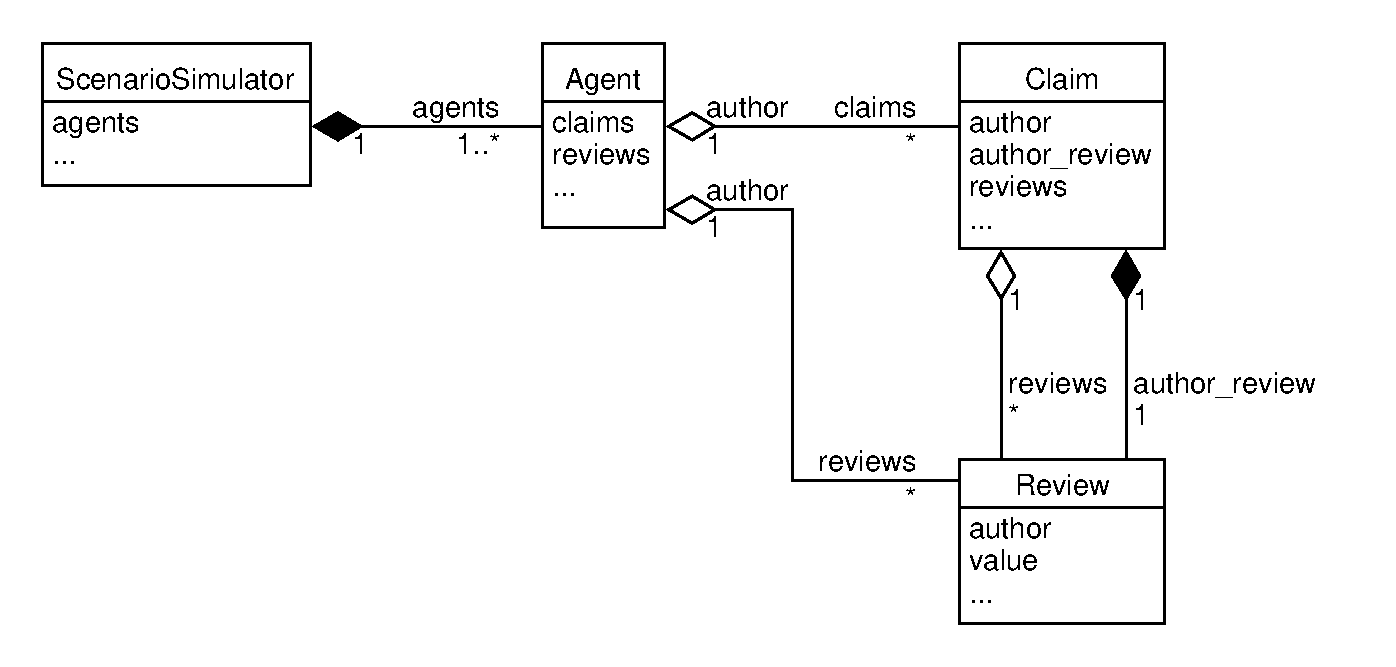
\includegraphics[width=1\linewidth]	{../uml/agents_data_structure.pdf}
    \caption{
	UML class diagram detailing how data is stored during simulation.
	\emph{Agent} instances representing agents in the scenario are held in a list in \emph{ScenarioSimulator}.
	Each agent holds a number of claims made by that agent.
	Claims have exactly one \gls{author_review} attached to them.
	Other reviews are held in a list in \emph{Claim}.
	Agents also hold the reviews made by them in a list of their own.
	Claims and reviews link back to their authors with weak references.
    }
    \label{fig:agents_data_structure}
  \end{center}
\end{figure}

\subsubsection{Passing the Data}
All data reflects the latest state during simulation.
Improvements act on this data and modify it accordingly.
For example, the aging improvement removes old claims directly from the live agents list stored in \emph{ScenarioSimulator}.

This approach has disadvantages with certain improvements that make only temporary changes to claims or reviews.
For example, an outlier filtering removes extreme opinions.
Once majority opinion shifts toward the opinions previously deemed an outlier, they need to be re-added since they are no longer outlier.
With the approach used, it has to remove reviews from the two lists in agent and claim, and then store them until they are to be re-added.
This is not an issue in itself, because improvement handlers are implemented as classes and can store data.

Another drawback shows itself at the end of the simulation.
Here, the original unimproved state of the data that includes removed or disabled parts is not available for processing and evaluation.
Metrics solve this issue however.
This way partly the reason for how metrics were implemented as they are, called on various points of the simulation.
At each simulation event where metrics are called, they export the needed data.

The advantage of keeping the data structure always in the live state is that it remains free of clutter.
Apart from this, simulation time is not increased by having to iterate through and check for inactive or removed objects.

\subsubsection{Alternative Storage Approaches}

Some alternative approaches were also considered.
One alternative would have been storing the effects of improvements within the data structure with flags.
For example, aging would add a flag \lstinline{counted=False} to claims deemed too old.
This would be good for improvements like outlier filtering, that take objects out of consideration and possibly re-add it later.
Outlier filtering would only need to change a flag back to \lstinline{True} to re-enable a review or claim.

One drawback of this would be that all the temporarily removed data objects would still remain in the live data lists.
They would be iterated over many times during rounds, increasing simulation time.
To prevent this, removed objects could also be stored in separate lists.
In this case however, the approach is mostly identical to what was implemented anyway.

Another drawback is that the simulator needs to check for the various flags introduced.
There can be many flags, like \lstinline{counted}, \lstinline{removed}, \lstinline{boosted}, \lstinline{weakened} etc.
Once checks for flags are built into Pyrepsys, improvements would no longer be modular, because code specifically tailored to them would remain in the simulator constantly.

\vspace{6pt}

Another approach to organize the data would have been storing different states of the data.
For example, also store a version without any modification by improvements, just the raw data that was generated by agents.
In parallel, the actively improved version is also stored.

Generally, such data duplication is disadvantageous.
It takes more memory and is harder to manage.
Processing time also increases.
Apart from this, the unimproved raw data would tell a false picture.
For example, it would store all claims for all rounds, without telling some claims were removed by aging.
Or store all reviews for all rounds, even though a couple of them would have been filtered inactive for some rounds.
Improvements also have a feedback effect on the data generated in subsequent rounds.
For example, a review of a claim removed by filtering can possibly change how another agent rates the claim.
Only seeing the raw data that includes the filtered review, the decision (rating) process of the other agent could not be reconstructed properly.

So the two datasets could be analyzed strictly together only.
This would be problematic, since the live view would hold the data from the last round only.
There is no information about what happened when in rounds before the last.

\subsubsection{Data in Metrics}
Metrics are a special case of data storage.
As mentioned above, one of the reasons they came to be was that data often needs to be saved along the time domain.
An example is following the change of reputations in every round.
For this purpose, metrics are hooked into points of simulation like the end of rounds and end of scenarios.
These are called simulation events.
With this, any snapshot of the data is possible.

Metrics get access to simulation data structure discussed above.
Specifically, they receive the list of agents stored by \emph{ScenarioSimulator}.
From it, they are free to take and store data as they wish.
Because metrics are implemented as classes, they can store data of their own.

The drawback of this approach is that data is stored multiple times after all, in the metrics.
This takes up some additional memory.
However, metrics rarely store a copy of the raw data only.
Most often they do some kind of (pre)processing already at storage.
For example, calculate an average of something per round, or make aggregates of agent data, etc.
This justifies their separate data storing.
When time-based raw data does need to be stored by metrics, it is only done on a need basis.
Meaning when that metric is not needed, it is turned off and the system is no longer strained by holding unneeded data.


\subsection{Internal and Agent-Exposed Values}\label{sec:i_ae_reprepentation}
Reviews, claim qualities and reputations can take up any value depending on the reputation scheme.
The simplest case is when reviews are either positive or negative.
This might be represented as 0 and 1.
In other cases, discrete values are needed, like \emph{good}, \emph{ok} and \emph{bad}.
Finally another common case is when values are integers in a range.
For example, the 5-star system using 1, 2, 3, 4 and 5 as possible values is common.
By default, Pyrepsys also uses this approach with values between 1 and 9.
This is however, decided by the scenario configuration.

The need for flexibility in reputation schemes necessitates a generic storage solution of values in Pyrepsys.
This is the reason values are stored differently internally than they are displayed and used by agents.
\Gls{ae_representation} is when a value is in the state facing the agents, the reputation system and display or export functions.
This is what is mentioned in examples above.
\Gls{i_representation} is the way Pyrepsys stores values in the internal data structures.

Internally stored values are in the range [0,~1].
Agent-exposed values are controlled by scenario settings.
The scenario configuration parameters \emph{MIN\_RATING} and \emph{MAX\_RATING} determine the possible range.
In the code, whenever a variable stores internal values, it end with '\texttt{\_i}', while variables of agent-exposed values end with '\texttt{\_ae}'.

Every time a value is fetched from or is saved to another state of representation, it is converted.
Conversion is done by two functions in the \texttt{helpers} module. 
These are \lstinline{agent_to_internal()} and \lstinline{internal_to_agent()}.
Both have a shorter alias in the form of \lstinline{a2i()} and \lstinline{i2a()}.
These functions take a single value $v$ as input and return the converted equivalent in the other representation. 
Conversion follows equations \ref{eq:a2i} and \ref{eq:i2a}.
\begin{equation}\label{eq:a2i}
v_{internal} = \frac{v_{ae} - \mathrm{minimum~rating}}{\mathrm{\gls{rating_span}}}
\end{equation}
\begin{equation}\label{eq:i2a}
v_{agent~exposed} = (\mathrm{minimum~rating}) + (\mathrm{\gls{rating_span}}) * v_{i}
\end{equation}

Used together with resolution, it is possible to reproduce schemes like the example ones at the beginning of this section.
See sections \ref{sec:approach_resolution} and \ref{sec:impl_resolution} for details on resolution handling.
Table~\ref{tab:rating_scheme_examples_pyrepsys_config} shows how the scenario should be configured for common schemes.
Agent-exposed representation gives numeric values even when they are meant as labels or other non-numeric choices.
In these cases, behavior and reputation strategies and metrics have to take care of interpreting them as such.

\begin{table}[tbp]
\centering
\begin{tabular}{@{}llccll@{}}
\toprule
\multirow{2}{*}[-0.2em]{\textbf{Scheme}} & \multirow{2}{*}[-0.2em]{\textbf{Rate Values}} & \multicolumn{2}{c}{\textbf{Rating Settings}} & \multicolumn{2}{c}{\textbf{Representations}} \\ \cmidrule(lr){3-4} \cmidrule(lr){5-6} 
                        &                                  & \textbf{Range}    & \textbf{Resolution} & \textbf{Internal}    & \textbf{External}   \\ \midrule
Binary          & +, -                     & {[}0,1{]}                & 1               & 0, 1 & 0, 1           \\
Labels & good, ok, bad       & {[}1,3{]}                & 1               & 0, 0.5, 1 & 1, 2, 3          \\
5-star          & 1, 2, 3, 4, 5            & {[}1,5{]}                & 1               & 0, 0.25, 0.5, 0.75, 1 & 1, 2, 3, 4, 5            \\ 
Precise & 1, 1.1 ... 4.9, 5 & {[}1,5{]}                & 0.1         & 0, 0.025 ... 0.975, 1 & 1, 1.1 ... 4.9, 5         \\
\bottomrule
\end{tabular}
\caption{
	Example rating schemes and Pyrepsys scenario configuration implementing them.
	The last two columns show how possible values are represented in the system.
	Using rating range and review resolution all common schemes can be configured.
	External refers to agent-exposed representation.
}
\label{tab:rating_scheme_examples_pyrepsys_config}
\end{table}


\subsection{Resolution}\label{sec:impl_resolution}

Resolution settings control what exact values are allowed for select variables during simulation.
This section discusses implementation details.
See section~\ref{sec:approach_resolution} for conceptual discussion of resolutions.

\subsubsection{Domains and Conversion Points}
Pyrepsys defines two resolution domains.
Each of these represent a resolution constraint for a part of the claiming, rating or reputation process.
When a value that is part of a process enters a domain, it is converted to the configured resolution.
Figure~\ref{fig:resolution_domains} shows which domains apply to what parts of the claiming and rating processes.

Domains determine the smallest allowed step for selected variable values.
The two scenario parameters that control the two domains are \texttt{REVIEW\_RESOLUTION} for reviews and \texttt{MEASURED\_CLAIM\_RESOLUTION} for measurements.
Both of these expect the value of the smallest allowed step given in \gls{ae_representation}.

There are three transformation points as also seen on figure~\ref{fig:resolution_domains}.
\begin{enumerate}
    \item on the result of a claim quality measurement, before the agent sees the measurement in its rating or distort strategy
    \item after the execution of a rating strategy on the returned review, before publishing the review
    \item after the execution of a distort strategy on the returned distorted quality, before publishing as author's review
\end{enumerate}

Reviews and distorted qualities are results of the customizable behavior strategies of agents. 
Conversion of these results is done without any punishment for agents that do not prepare their values for the configured review resolution.
All reviews are saved with this resolution, whether an agent's review or a claimer's author review.

Code implementing resolution handling is found in the \texttt{helpers} module.

\subsubsection{Resolution Conversion}

When a value that is part of a process enters a domain, it is converted to the configured resolution.
The main function for converting between resolution domains is \lstinline{convert_resolution()}.
It expects two arguments.
First, \texttt{number} holds the value to be converted.
Second, \texttt{target\_resolution\_domain} gives which resolution it should convert to.
This is given in the form of an enum defined in \texttt{helper\_types}.
The purpose of \lstinline{convert_resolution()} is to call the \lstinline{find_nearest_step()} with the appropriate arguments to find which step the value to convert falls nearest to.

The function \lstinline{find_nearest_step()} accepts \texttt{number} holding the value to be converted and \texttt{steps\_sorted\_list}, a list sorted by ascending order and containing all the allowed steps of the chosen resolution domain.
It is this function's job to effectively convert to the new resolution by selecting a possible step from the list based on the value of \texttt{number}.
For this, it uses a bisection algorithm \lstinline{bisect_left} from Python's \texttt{bisect} module.

Left bisection efficiently searches for an element in a sorted list.
Originally it is meant to be used for efficiently inserting new items into a sorted list.
Given a sorted list and a new item, bisect returns the index where the item should be inserted into the list to keep it sorted.
Since it uses binary search for finding this, its efficiency is $O(logN)$.
The difference between left or right bisection is if the element to insert is already in the list, should the returned insertion index be left or right of the existing equivalent element(s).

With the point of a would-be insertion found, \lstinline{find_nearest_step()} decides on the returned resolution step.
The index returned by left bisection is denoted by \lstinline{i}.
If the input \texttt{number} coincides with resolution step \lstinline{steps_sorted_list[i]}, that is returned.
If not, then \texttt{number} is between \lstinline{steps_sorted_list[i]} and \lstinline{steps_sorted_list[i-1]}.
The distances from both are calculated as seen below.

\begin{lstlisting}
diff_left = round(abs( steps_sorted_list[i-1] - number ), 8)
diff_right = round(abs( steps_sorted_list[i] - number ), 8)
\end{lstlisting}

Rounding is needed to correct small floating-point errors that can result from working with small numbers.
The step with the smaller distance is returned.
If the distances are equal, the larger, right-neighboring step is returned.

\subsubsection{Creating Resolution Steps}\label{sec:impl_create_steps}

Ordered lists of possible resolution steps are created for every resolution domain.
These are called step lists or resolution ladders.
The step lists are sorted by ascending order and are created during scenario configuration by the function \lstinline{_configure_system_resolutions()} in the \lstinline{helpers} module.
The method is simply starts with the smallest value, increments it with the resolution's step and adds it to the step ladder.
This is repeated until the maximum allowed value is reached.
Each step list is stored in a module-level variable in \lstinline{helpers}.

The function \lstinline{_configure_system_resolutions()} is an exception from all others related to configuration, which are located in the \lstinline{config} module in the \emph{Configurator} class.
The reason for putting this function in \lstinline{helpers} instead of \lstinline{config} is to avoid a circular import dependency between the two modules.
An alternative solution was to keep the functionality in the \emph{Configurator} class.
In this case, the resolution steps would have to be requested via the \lstinline{get()} method of \emph{Configurator}, or with a similar call.
This adds an overhead, and since resolution conversion is a very common operation, so it can build up to a noticeable factor.
Because of this, the resolution ladders are kept locally in \lstinline{helpers}.

To allow (re-)calculation of the resolution steps every time the scenario configuration changes, \emph{Configurator} must let the \lstinline{helpers} module know when this happens.
This is solved with callbacks from \emph{Configurator}.
The function for calculating resolution ladders is registered with \emph{Configurator}, which calls it every time the scenario configuration is updated.
For more discussion on configuration updated callbacks, see section~\ref{sec:config_update_callbacks}.

\begin{figure}[tbp]
  \begin{center}
        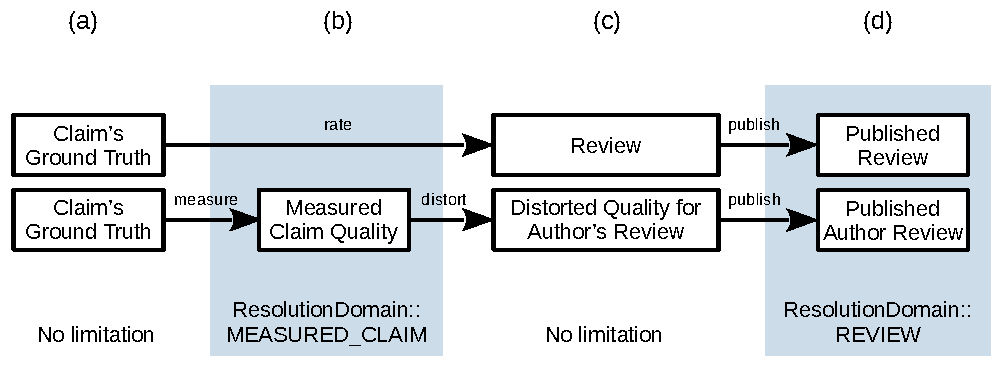
\includegraphics[width=1\linewidth]	{../images/resolution_domains-crop.pdf}
    \caption{
    Resolution domains in various stages of rating (top) and claiming (bottom).
    (a) Ground truths have no limitation and can take up any value within the \gls{rating_span}, stored as \gls{i_representation}.
    (b) Claim quality measurements are produced in the \emph{measured claim resolution domain}.
    (c) In their distorting or rating strategies, agents can compute an output without regard to resolution constraints.
    (d) Once the produced values are published, they are converted into the \emph{review resolution domain}.
    }
    \label{fig:resolution_domains}
  \end{center}
\end{figure}



% --------------------------------------------------------------
\section{Random Number Generation}\label{sec:impl_rng}
% --------------------------------------------------------------

Python's \lstinline{random} module is used for generating random numbers.
Many parts of Pyrepsys uses random numbers for simulation.
These include:
\begin{itemize}
	\item Ground truth of new claims
	\item Random error on claim quality measurements
	\item Checks against an agent's claim or rate probability
	\item Some agent behavior strategies
\end{itemize}

In order to facilitate comparability and repeatability of simulations, Pyrepsys implements repeatable random number generation.
Python's \lstinline{random} rolls its internal state every time a random number is taken from it.
If the state of the generator is known and can be restored, random number sequences can be recreated.
Such sequence of random numbers are called random chains here.

Repeating the chain of a random number generator is possible by seeding it.
Scenarios provide a configuration parameter called \lstinline{seed} for this purpose.
The class \emph{ScenarioSimulator} owns an instance of the random number generator created with the \lstinline{random} Python module.
Before simulation of a scenario, the generator is seeded with the above parameter.
This generator provides the so-called \gls{main_rng_chain}.
It serves random values for checks and uses where the same number and type of random value is needed regardless of what execution path the simulation takes.
These are for example checks whether agents will claim or not, provide a review or not, and providing random seeds for throwaway random chains.

\Glspl{branchoff_rng_chain} or throwaway chains are supplementary random number sequences.
These are used when it is not known in advance how many or what type of random values are needed, or whether any will be needed at all.
Such cases are claiming and rating randoms, or agent behavior strategies.

Throwaway chains are made by branching-off the main chain.
That means a random value is rolled from the main generator, and used as seed for the throwaway chain.
To provide a constant usage of the main chain, every time there is a possibility that a branch-off chain will be needed, a random number will be generated for its seed.
This way the chain is used equally regardless of the scenario's settings.

An example illustrating the purpose of the two random chains is claiming.
Claiming requires three random values: 
\begin{itemize}
	\item one for the claim probability check to see if the agent will attempt a claim
	\item one for generating a ground truth (quality) in the new claim
	\item one for the measurement error when the agent assesses the claim's quality
\end{itemize}
The first one of these must be generated whether the agent claims or not.
The second two only if the check to claim succeeds and claiming is attempted.
Changing the number of agents or agent's claim probabilities would modify which agents enter the the claiming process, and so the agents claiming afterward the shift would get different random values than before.
To prevent this, each claim opportunity uses exactly two random values off the main chain: one for the probability check, and another as a seed for the branch-off random chain.
If the agent passes the probability check, the generated seed is used to create the branch-off random sequence.
The random values for the new claim's quality and the measurement error are taken from this throwaway chain, which is destroyed after the claiming.
In this manner, all agents receive the same inputs from the simulator even between scenarios, provided that the order of the agents stays the same.



% --------------------------------------------------------------
\section{Configuration}\label{sec:impl_config}
% --------------------------------------------------------------

This section discusses topics related to configuration in Pyrepsys.
It also covers some scenario parameters, but not all.
For a usage-oriented description of every possible scenario parameter, see appendix~\ref{appendix:scenarios} instead.


\subsection{Scenario Definition}
\Glspl{scenario} are expected as \texttt{.yaml} files located in the \texttt{scenarios} folder.
Each file contains a list of parameters in yaml format, telling what the scenario is about.
Parameters include the reputation strategy, used improvement handlers, agents, enabled metrics, resolution, rating range, the initial seed and other settings.

%Pyrepsys allows describing scenarios without a full specification.
%This means not all needed parameters are listed, just some selected ones.
%The missing parameters are taken from a default scenario configuration.
%This is useful when the effect of one or more parameter changes are needed, since those can be simply listed alone in their scenario configuration.
%For all conceptual discussions, a scenario refers to all the simulation environment fully specified, regardless of where they come from in the implementation.
Scenario files can either be fully or partially defined.
Full definition requires the scenario give an explicit value for all possible parameters.
Partially defined scenarios contain only a subset of all settings.

Scenario files can fill two different roles when running Pyrepsys.
First, regular scenarios are the separate simulation units that will be simulated after each other.
These are given as a list to simulate, typically more than one per invocation.
Second, the default scenario is used as a fallback for parameters while simulating the list of regular scenarios.
Only one scenario file can be given as default scenario every Pyrepsys invocation.
The two kinds of scenarios form a two-level system.
Whenever a regular scenario is simulated and a parameter is requested, the system checks among the parameters from the scenario file.
This is called the active configuration.
If a parameter is not defined there because the scenario is not fully defined, then the default scenario serves as fallback.
The requested parameter is returned from the default configuration.
For this reason, the scenarios used as default scenario must always be fully defined.

Defining scenarios with this two-level configuration system is simpler.
Usually only one or at most a few parameters are varied between scenarios to see the isolated effect of the changes.
Here, the default scenario should contain the baseline values for scenario parameters, fully defined.
Then, each specific simulated scenario can be partially defined only containing parameters that differ from the default configuration.
Pyrepsys provides a scenario creator utility, which uses the same approach to create scenarios with combinations of given parameter values.
See appendix~\ref{appendix:sc} for documentation.

\subsection{Reading Scenario Files}
Reading configuration from scenario files to memory is done by the \emph{Configurator} class.
It provides two separate methods for reading active and default scenarios.
Both are wrappers for the same class method responsible for reading scenario files, named \lstinline{_config_from_file_to_memory()}.
After opening and reading the file contents, it calls on the third party \texttt{pyyaml} module to read the contents into a dictionary.
A name for the scenario is added to the dictionary by taking the filename without the \texttt{.yaml} extension.
The function also generated the hash of the scenario file it just read using the sha256 algorithm.
This will be logged to provide a quick check whether two scenarios of the same name contain the same settings.

\subsection{Configuration Storage Locations}
Multiple locations are responsible for storing configurations in Pyrepsys.
\emph{Configurator} is the main source of settings.
Apart from that, locally stored config collections also exists, and there is one local configuration cache.

\subsubsection{Configurator}
\emph{Configurator} is located in the \texttt{config} module and is responsible for most configuration-related functionality.
Its main tasks are reading scenario files, preparing other modules and classes for simulation, and providing configuration parameters when requested.

The class method \lstinline{get()} can be used to request config values from \emph{Configurator}.
It takes an argument with the name of the config parameter.
This function implements the two-level configuration retrieval.
First the active config is checked, and then the default if the active configuration does not contain the requested parameter.

\emph{Configurator}'s storage of active scenario settings is changed between scenarios, while the default config remains the same for the whole duration of a Pyrepsys run.

\subsubsection{Local Configuration of Strategies and Handlers}\label{sec:local_config}
Some behavior or reputation strategies, improvement handlers or even metrics are parametrized and so can have configuration values attached to them.
An example for how these are defined in scenario files is found below.
\begin{lstlisting}
improvement_handlers:
  - name: "Aging"
    limit: 6
  - "Weights"
\end{lstlisting}
Here, aging is defined with one parameter called \texttt{limit}.
When configuration is attached in this way, the original param value is replaced with a dictionary, and the \texttt{name} param is used to hold what was just a string before.
For comparison, the \texttt{Weights} improvement handler uses no parameters in the above example, so only the implementig class' name is needed as a string.

Strategies, handlers or metrics that are extended with parameters like this are interpreted by the \emph{Configurator} class in a method called \lstinline{_unpack_extended_config_list()}.
After an instance of the appropriate class is created, it receives a dictionary containing its parameters if there are any.
The storage solution is the class \emph{LocalConfig}, from which all strategies, handlers and metrics inherit.
This class provides a method similar to \emph{Configurator}'s \lstinline{get()} for accessing the local config.
These are then accessible from within the class methods of strategies, handlers or metrics.

Storing these parameters with the class instances instead of a central repository like \emph{Configurator} allows instantiation of different versions of the same class.
Simply the local config needs to be specified with different values.

\subsubsection{Configuration Caches}
There is one occasion where a Pyrepsys module uses a local cache for scenario configuration that normally would be requested from \emph{Configurator}.
This caching appears in the \texttt{helpers} module.
Before its introduction, the conversion functions between \gls{i_representation} and \gls{ae_representation} made multiple config param requests each.
These are very frequently used functions, because they are called every time an internally stored value is fetched, or when an agent-generated value is stored.
While \emph{Configurator}'s \lstinline{get()} is fast, the sheer amount of calls made incurred a noticeable overhead.
When this local cache was introduced, it resulted around 70\% improvement in the cumulative time spent in the function that converts from internal to agent-exposed representation.
This can mean around minute that was shaved off. 
Other functions in helpers also benefit from speed improvement, albeit to a lesser degree.

Caching works by storing needed configuration parameters and precalculated values in the \texttt{helpers} module.
Module functions can then access the cache dictionary instead of making a request from the \texttt{config} module.
\emph{Configurator} updates the cache via a callback each time the scenario configuration is modified.


\subsection{Update Callbacks}\label{sec:config_update_callbacks}
\emph{Configurator} allows registering callbacks for configuration changes.
These are called every time the default or active scenario configuration changes.
Other parts of Pyrepsys can use this to be notified of changes in configuration.

The method to register the callback functions is \lstinline{register_config_updated_callback()}.
Every time a new scenario file was read and parsed, \emph{Configurator} executes all registered callbacks.
Update callbacks are used by the local config cache in \texttt{helpers} and the resolution step ladder creator method.
Refer to section~\ref{sec:impl_create_steps} for why resolution handling is solved this way.


\subsection{Setting Up Simulations}
The \texttt{main} module serves as an entry point and coordinates the Pyrepsys classes to perform simulations.
After preparatory tasks like logging setup and creating the output folder, instances of \emph{ScenarioSimulator}, \emph{ResultsProcessor} and \emph{Instantiator} are created.
The system-wide \emph{Configurator} instance is also requested.
The \texttt{config} package provides \lstinline{getConfigurator()}, which returns the same instance of \emph{Configurator} every time it is called.
\emph{ScenarioSimulator} receives \emph{ResultsProcessor}, the configurator gets the \emph{Instantiator} instance and the output directory path.

Now, the scenario files can be read and the objects can be configured.
First, the default scenario settings are read.
Then, for each scenario, its file is read, \emph{ScenarioSimulator} is configured, \emph{ResultsProcessor} is configured, then begins the simulation.
This repeats until all scenarios were simulated.

The scenario simulator's setup is divided into three parts: improvement handlers, reputation strategy and agents.

\subsubsection{Reputation Strategy and Improvement Handlers}
Reputation strategy and improvements have a similar setup.
First, the params storing them are requested.
Then, a method called \lstinline{_unpack_extended_config_entry()} parses parameters that are extended with local configuration described in section~\ref{sec:local_config}.
\emph{Instantiator} is used to create reputation and improvement handler object instances.
The instances receive their local config is any was set for them, and they are assigned to the \emph{ScenarioSimulator}.
For the improvement handlers, the improvement chain is tied together in order of appearance in the scenario file, and the scenario simulator only receives the first handler.

\subsubsection{Agents}
For setting up agents, the agent base behavior definitions also need to be parsed first.
Base behaviors are template settings for agent definitions, defined in scenario files under the parameter \lstinline{agent_base_behaviors}.
Each of them must contain all possible agent parameters, along with the base behavior's name.
For example:
\begin{lstlisting}
agent_base_behaviors:
  - name: 				"HonestAccurateRater"
    distort_strategy: 	"DistortDoNothingStrategy"
    rate_strategy: 		"RateFromOwnExperience"
    claim_range: 		[0, 1]
    claim_probability: 	0
    rate_probability: 	1
    claim_truth_assessment_inaccuracy: 0.0625
\end{lstlisting}
Base behaviors can then be used when defining agents. Below, the above definition is used to define two agent types. Both of them will have 10 agents created of the type. The second type overwrites the base behavior's \lstinline{claim_probability} of 0 with 0.2.
\begin{lstlisting}
agents:
  - amount: 			10
  	base_behavior: 		"HonestAccurateRater"
  - amount: 			10
  	base_behavior: 		"HonestAccurateRater"
  	claim_probability: 	0.2    # overwrite claim% from the base behavior
\end{lstlisting}
The typical usage method for base behaviors is defining a set of base behaviors in the default scenario's file, and then using these definitions in other scenario files that will be simulated.
Otherwise, \lstinline{agent_base_behaviors} also adheres to the two-level configuration system.
If it is re-defined in an active scenario's file, that definition overwrites the one in the default scenario settings.

Each agent type's rate and distort strategies are created in a similar manner to reputation strategies and improvement handlers.
The local config parameter extensions are parsed, then instances are created.
With the agent's configuration parameters and behavior strategies ready, the \emph{Agent} instances are created.

This is done by \emph{ScenarioSimulator}, with its method for this task called \lstinline{create_agents()}.
Agent objects are saved by scenario simulator into the agents list.

\subsubsection{Metrics and ResultsProcessor}
Metric instances are special in the regard that they are persistent between all simulated scenarios of a Pyrepsys invocation.
This is because metrics usually compare multiple scenarios, and they need to be able to collect and store data from each of them.
\emph{ResultsProcessor} stores metric instances for this reason.

During configuration, \emph{Configurator} checks if \emph{ResultsProcessor} already stores instances of the listed metrics of scenarios.
If not yet, the same process from earlier sections involving local configs and the \emph{Instantiatior} is used to create the missing metric instances.
\emph{ResultsProcessor} receives them and will keep them until Pyrepsys terminates.

Including or excluding a metric from data collection during a scenario is determined by the \lstinline{metrics} parameter in scenario files.
The two-level system of default and active configurations applies to it like to any other parameter.
The typical usage is listing metrics used in the default scenario's file, and not defining any metrics in the simulated scenarios.
This results in the same default metrics being used for all scenarios.
If any scenario defines the \lstinline{metrics} parameter, \emph{only the metrics found in this definition} will be used for the scenario, since it completely overwrites the one in the default.
To add an extra metric along the defaults to a scenario, it needs to be listed explicitly with the default metrics as well.
To exclude one compared to the default definition, all other not-excluded metrics need to be listed.



% --------------------------------------------------------------
\section{Results Processing}\label{sec:impl_results_processing}
% --------------------------------------------------------------
Pyrepsys offers optional built-in results processing to form a full pipeline from simulation to data analysis and visualization.
The \lstinline{results_processor} and \lstinline{metrics} modules can collect, process and export simulation data as graphs or tables.
\emph{Metric} classes define what data is collected, and how it is processed and exported.
\emph{ResultsProcessor} contains the metrics, notifies them of events and funnels simulation data to them.
Together, metrics and \emph{ResultsProcessor} form a publish-subscribe architecture.
The UML diagram of these classes is found in figure~\ref{fig:reproc_metrics}.


\subsection{Simulation Events}

Pyrepsys defines four simulation events as listed in table~\ref{tab:simulation_events}.
Each time execution reaches one, the event is triggered by notifying the results processor of it.
Then, \emph{ResultsProcessor} notifies the metrics of events that concerns them.

Two events have fixed consequences.
The \lstinline{BEGIN_SCENARIO} event calls every active metric's \lstinline{prepare_new_scenario()} method, which is used to make preparations before the scenario starts.
\lstinline{END_OF_SCENARIO} calls the \lstinline{export()} method of active metrics, which is used to make post-processing on the data, assemble graphs or tables, and export them into files.

The two other events are \lstinline{END_OR_ROUND} and \lstinline{END_OR_SCENARIO}.
Each activated metric subscribes to none, just one or both of these two.
Whenever these events trigger, the \lstinline{calculate()} method of subscribed metrics is called by \emph{ResultsProcessor}.
This is the time metrics can save data from the simulation system and do pre-processing on it.

Which of the two events a metric subscribes to is determined by what kind of reporting the metric does.
In any case, simulation data is passed for \lstinline{calculate()} for both events in the form of the agents list, the same one saved by \emph{ScenarioSimulator}.
Depending on which event it is, the just ended round's number or the ended scenario's name is also passed.

\begin{table}[tbp]
\centering
\begin{tabular}{ll}
\toprule
\textbf{Event}        & \textbf{Called Metric Method} \\ \midrule
BEGIN\_SCENARIO       & \texttt{prepare\_new\_scenario() } \\
END\_OF\_ROUND        & \texttt{calculate()} if registered \\
END\_OF\_SCENARIO     & \texttt{calculate()} if registered \\
END\_OF\_SIMULATION   &  \texttt{export()} \\
\bottomrule
\end{tabular}
\caption{
	Simulation events in Pyrepsys.
	\emph{ResultsProcessor} is notified of events from other parts of the code.
	It notifies metrics based on what event was triggered and which metrics are active.
	The second column shows which methods of active metrics are called.
}
\label{tab:simulation_events}
\end{table}


\subsection{Metrics}

Generally there are two types of metrics: data exporters and graph plotters.
The distinction is not strict however, and metrics can even have both functions at the same time.
It makes sense to divide metrics along what kind of reporting they do.
When a metric calculates a specific kind of value, statistic or aggregate, it can make sense to produce graphs and data exports from the same metric, since the data is available anyway.

Every metric is defined as a child of the abstract \emph{metrics::Metric} class, as seen in figure~\ref{fig:reproc_metrics}.
Then, selecting metrics for usage is done through the scenario configuration by giving its classname.
The initialization method contains a metric's name and its events of interests.
Additionally, every metric implements at least the three previously discussed functions.
Graph plotting metrics in Pyrepsys use \texttt{matplotlib}, while data exporters use Python's \texttt{csv} module.
Exported files are saved to an invocation-specific output directory called the \gls{artifacts_dir} by default.

Using metrics with Pyrepsys is optional.
The costs of using them is the extra memory needed for storing collected data, and the additional processing time for dealing with the data and creating the export formats.
The memory footprint obviously depends on how big of a simulation data is amassed and how many separate metrics store parts from it.
Processing time spent on metrics was observed to be tens of seconds when simulation takes a few minutes.

The benefit of metrics is the convenience of automatic reports and graphs exported based on simulation data.
Flexibility and extendability is also fulfilled.
Adding new metrics is as easy as with any other behavior or reputation strategy, or improvement handler.

\begin{figure}[tbp]
  \begin{center}
        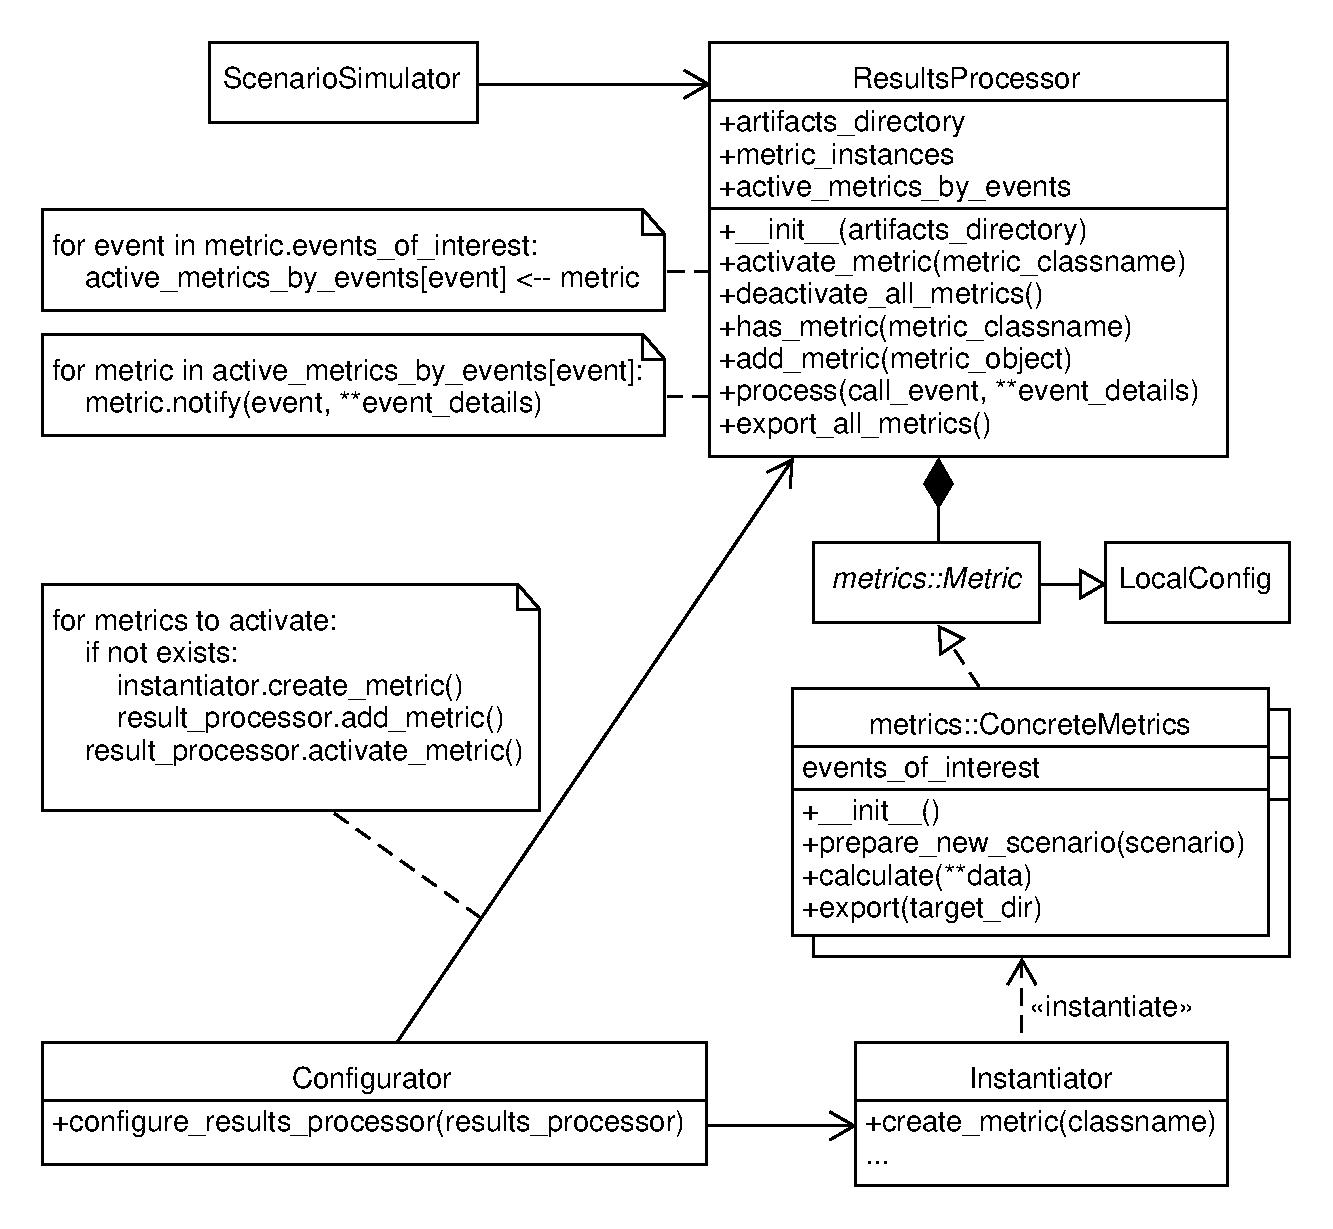
\includegraphics[width=1\linewidth]	{../uml/reproc_metrics.pdf}
    \caption{
	UML class diagram of the results processor and metrics.
	Metric instances are created by \emph{Configurator} via \emph{Instantiator}.
	\emph{ResultsProcessor} registers metrics according to what event they are listening to.
	\emph{ScenarioSimulator} and the \lstinline{main} package trigger events on the results processor.
	Metrics are notified of events that interest them.
	\emph{LocalConfig} provides custom configuration for each individual metric.
	This is discussed in section~\ref{sec:local_config}.
    }
    \label{fig:reproc_metrics}
  \end{center}
\end{figure}



% --------------------------------------------------------------
\section{Other Facilities}\label{sec:impl_misc}
% --------------------------------------------------------------

\subsection{Automated Self-Testing}
Pyrepsys contains an automated testing suite.
It can be used to verify the integrity of functionality under the test coverage.
Tests can also be added to perform sanity checks of specific components, like metrics.
Such tests contain scenario configuration that is known to produce an expected and explainable results.
Finally, the test suite contains tests that profile and benchmark the simulator.
Using these the most time-consuming parts of the simulation can be identified.

Testautomation is provided by Pytest.
Tests reside in the \texttt{tests} directory in Python files.
Each of them is a function and are found automatically by Pytest.
To allow some control over what tests to run, Pyrepsys uses Pytest's mark feature.
Some tests are marked with the identifiers found in table~\ref{tab:pytest_marks}.

\begin{table}[tbp]
\centering
\begin{tabular}{ll}
\toprule
\textbf{Mark}        & \textbf{Meaning} \\ \midrule
perf       & Test does profiling or is a benchmark \\
manual     & Test needs manual evaluation of results \\
long       & Test takes a longer time than most others \\
\bottomrule
\end{tabular}
\caption{
	Pytest test markers in Pyrepsys.
	Relevant tests are flagged with them.
	Marks can be used to select which tests to run or exclude from running.
}
\label{tab:pytest_marks}
\end{table}


\subsection{Logging}
Pyrepsys logs notable events and information in a logfile saved to the \gls{artifacts_dir}.
This is implemented using Python's \lstinline{logging} module.

Logging is set up by \texttt{pyrepsys.main}.
Messages are logged into the logfile called \texttt{simulation.log}.
They are also displayed on the console in a shortened format.
Each Pyrepsys module gets its own logger with the \lstinline{logging.getLogger()} method.
It returns the logger after the \texttt{name} parameter provided to it, which is chosen as the name of each Pyrepsys module.

Messages of different severity are logged, including debug, info, warning and error.
By default, only info level messages or more severe are displayed.
If debug messages are needed, the default level can be overwritten in the \texttt{pyrepsys.main} module.
It is also possible to change the severity of selected Pyrepsys modules only.
This is beneficial when debugging a specific module.




% CHAPTER ######################################################################
\chapter{Evaluation} \label{chap:evaluation}
% ##############################################################################


% --------------------------------------------------------------
\section{Metrics}\label{sec:metrics}
% --------------------------------------------------------------
%Metrics: First define which quantities you will measure and why you chose those.

Effectiveness is measured as a global, system-wide accuracy, as opposed to an agent-utility approach.
This is chosen because measuring idividual agent's success makes less sense, since agents can not decide who they transact with.

The main metric for system accuracy is reputation scores compared to claimer's inaccuracy.
Claimers who publish accurate and reliable author's reviews should have a good reputation, while, inaccurate author's reviews should result in a lower reputation.
This way, an ideal linear relationship exists between inaccuracy and reputation, where the lowest possible claiming inaccuracy should map to the highest reputation, while the theoretical largest inaccuracy in the worst possible reputation.
This ideal line is shown as a dashed diagonal in plots of this metric.
If an agent is above the line, it managed to cheat the system by getting a better reputation than its inaccuracy and honesty would proportionally warrant.
If under, the agent is punished harder than it should be under straight proportions.

Total claiming inaccuracy is determined by two factors: measurement inaccuracy and distortion.
Since measurement is not under the agent's control, it is also called the involuntary inaccuracy.
Distortion is fully each agent's doing, so it is voluntary and also called dishonesty.
\begin{equation}
\text{Total Claiming Inaccuracy} = \text{Measurement Inaccuracy} + \text{Dishonesty}
\end{equation}
This is computable for a claim $C_A$ made by agent $A$ using the claim's author review and its \gls{gr_truth}.
\begin{equation}
\text{Total Claiming Inaccuracy}(C) = \left| Q_{true,C_{A}} - R_{authorA,C_{A}} \right|
\end{equation}
Averaging every claim of an agent gives the \emph{Average Total Claiming Inaccuracy} of that agent.

\vspace{6pt}

\emph{Average Inaccuracy of Raters} measures how close regular reviews fall to the ground truths of rated claims.
It is calculated as
\begin{equation}
\frac{\sum_{C\in\text{all claims}}({(\text{average of review on }C) - Q_{true,C})}}{\text{number of all claims}}
\end{equation}

This metric is most influenced by the setup of agents and their behavior strategies.
For this reason it can be used less to judge the effectiveness of reputation or improvement schemes, and more to see how the agent population rates.
When more dishonest or malicious raters are present, this metric will indicate that with a larger average inaccuracy.



% --------------------------------------------------------------
\section{Setup}\label{sec:setup}
% --------------------------------------------------------------
%Setup: Clearly describe which method you use to obtain your values and how the setup looks like. It is probably one of three:
%    Analysis: provide a formal/mathematical analysis of your approach (and related work). Which models / equations do you use? Why? How? 
%    Simulation: Run your approach in a simulation framework. Which simulator (version) runs on which hardware (specs)? Which parameters? Why?
%    Experiment: Measure values from a real implementation. Which devices are used? Conditions? Parameters?

Experiments are set up and simulated with Pyrepsys.
Each one consists of multiple scenarios with one or two selected parameters that are varied.
Most other parameters are kept the same to allow clear comparison.
Fixed parameters are
\begin{itemize}
	\item rating range: $[1,9]$
	\item rating resolution: 1
	\item measurement resolution: 0.5
	\item reputation strategy: \lstinline{BasedOnAvgDifferenceOfClaimsAndReviewsWithWeight}
	\item initial reputation: 5
	\item number of rounds: 80
	\item seed: \lstinline{pyrepsys_random_seed}
\end{itemize}

\begin{table}[tbp]
\centering
% comment for the old, long table
%\begin{tabular}{lrrllll}
\begin{tabular}{@{}lll@{}}
\toprule
%\multirow{2}{*}[-0.2em]{\textbf{Base Behavior}} & \multirow{2}{*}[-0.2em]{\textbf{Rate\%}} & \multicolumn{2}{c}{\textbf{Claim}}            & \multirow{2}{*}[-0.2em]{\textbf{\acrshort{ctai}}} & \multicolumn{2}{c}{\textbf{Behavior}}             \\ \cmidrule(lr){3-4} \cmidrule(l){6-7} 
% &  & \textbf{\%} & \textbf{Range} &  & \textbf{Distort} & \textbf{Rate}  \\ \midrule
%\texttt{HonestClaimer} & 0.1 & 1 & [0.5,1] & 0.125 & \texttt{DoNothing} & \texttt{DoNothing} \\
%\texttt{DishonestClaimer} & 0.1 & 1 & [0.5,1] & 0.125 & \texttt{MaxSometimes} 50\% & \texttt{RateFromOwnExperience} \\
\multirow{2}{*}[-0.2em]{\textbf{Base Behavior}} & \multicolumn{2}{c}{\textbf{Behavior Strategy}} \\ \cmidrule(lr){2-3}
 & \multicolumn{1}{c}{\textbf{Distort}} & \multicolumn{1}{c}{\textbf{Rate}} \\ \midrule
\texttt{HonestClaimer} & \texttt{DoNothing} & \texttt{DoNothing} \\
\texttt{DishonestClaimer} & \texttt{MaxSometimes} (0.5) & \texttt{RateFromOwnExperience} \\
\texttt{HonestRater} & \texttt{DoNothing} & \texttt{LinearFromClaimerReputation} (7)\\
\texttt{InfluencedHonestRater} & \texttt{DoNothing} & \texttt{BetweenAuthorReviewAndExperience} \\
\texttt{MidrangeRater} & \texttt{DoNothing} & \texttt{Flatten} (0.5) \\
\texttt{MaliciousRater} & \texttt{DoNothing} & \texttt{RateInvertedSlope} \\
\texttt{HonestClaimerRater} & \texttt{DoNothing} & \texttt{RateFromOwnExperience} \\
\texttt{DishonestClaimerRater} & \texttt{MaxSometimes} (0.5) & \texttt{LowrateHonestClaimers} \\
\bottomrule
\end{tabular}
\caption{
	Agent base behaviors used as template in simulations.
	Values in parenthesis show parameters for behavior strategies that need them.
	\texttt{MaxSometimes} has \emph{chance} of claiming the highest quality.
}
\label{tab:agent_base_behaviors}
\end{table}

Varied parameters are the improvement techniques and agent population composition.
Agent base behaviors shown in table~\ref{tab:agent_base_behaviors} are defined as templates.
Apart from the behavior strategies, the default agent parameters are
\begin{itemize}
	\item \gls{ctai}: 0.125
	\item claim range: [0,1], or [0.5,1] for  \texttt{HonestClaimer} and \texttt{HonestClaimerRater}
	\item claim probability: 0.8 for claimers, 0 for only raters
	\item rate probability: 0.8 for raters, 0.1 for only claimers
\end{itemize}

Experiments are each identified with a letter.

\subsubsection{Experiment A: effect of aging}
This experiment varies two parameters, both over three possible settings, making nine scenarios total.
First, improvements are varied as 1) no improvements, 2) aging with limit 25 and 3) aging with limit 10.
Then, the number of \texttt{MaliciousRater} agents are varied as 1) none 2) 30 and 3) 60.
\texttt{HonestRater} and \texttt{MidrangeRater} extend the agent population so that there are always 60 raters with these two in equal numbers.
Lastly, all scenarios include 10 \texttt{HonestClaimer} and 10 \texttt{DishonestClaimer} agents.

\subsubsection{Experiment B: malicious raters}
In this experiment, the ratio of dishonest raters is increased gradually.
Since reputation calculation is based on the honesty of claim valuations in the form of author reviews, dishonest raters who otherwise never claim will not get a reputation adjustment.

The experiment has 10 \texttt{HonestClaimer} and 10 \texttt{DishonestClaimer} agents, and a total of 60 rater agents.
These are made up of 1) none 2) 20 3) 40 and 4) 60 \texttt{MaliciousRater} agents.
\texttt{HonestRater} and \texttt{MidrangeRater} agents fill the remaining rater spots equally, until all scenarios have 60 raters.

The four versions are simulated with and without the weights improvement enabled, totaling at 8 scenarios.

\subsubsection{Experiment C: dishonest claimers}
This experiment has three versions, each a sub-experiment.
The first one (C/I) increases the ratio of dishonest claimers.
All scenarios have 60 raters, 20 of each type: \texttt{HonestRater}, \texttt{MidrangeRater} and \texttt{InfluencedHonestRater}.
The \texttt{HonestClaimer} to \texttt{DishonestClaimer} ratio is changed as 1) 10:0 2) 8:2 3) 2:8 and 4) 0:10.
The weighted and weightless versions are simulated additionally, totaling at 8 scenarios.

Since a third of the agents are influenced by author reviews in their rating decisions, claimers are expected to be able to manipulate these agents into a better rating than the claim's deserved quality.
However, the other agents are also honest and quite numerous, so combined they are expected to keep the dishonest claimers at bay.

The second (C/II) experiment has the rater types \texttt{HonestRater} and \texttt{MidrangeRater} removed, so only 20 \texttt{InfluencedHonestRater} remain as raters.
Compared to (C/I), the rater, or consumer agent population becomes more susceptible to influence.
This means they take author reviews of claims more seriously overall.
These agents are expected to be more easily manipulated, so dishonest claimers can possibly get a better reputation than before.

The third (C/III) version fixes the ratio of honest and dishonest claimers, 10 agents each type.
However, the 10 \texttt{DishonestClaimers} make dishonest claims increasingly often: 1) never 2) 50\% 3) 85\% and 4) 100\%.
This aims to find out whether there is an upper limit to frequency of dishonest claimers still tolerated.
Similar to (C/II) only 20 \texttt{InfluencedHonestRater} agents take part as raters.
However, their rate strategy is varied between 1) the usual for this agent type \texttt{RateBetweenAuthorReviewAndExperience} and 2) \texttt{RateFromOwnExperience}.
This changed the normally influencable raters to make rate decisions purely from their own opinion.

\subsubsection{Experiment D: effect of weights}
This experiment also has three sub-experiments and it aims to find out the effect of weights as improvement technique.
Because weights are calculated from reputations, both claimers and raters should get reputation adjusments.
For this, all agents need to be claimers, including the raters.
This is often not the case in reputation systems for people, but is common for algorithmic reputation environments, where agents are machines.

(D/I) uses \texttt{HonestClaimerRater} and \texttt{DishonestClaimerRater} agents in the numbers 1) 18:2 2) 14:6 3) 10:10 and 4) 2:18. Improvement techniques are varied as 1) Aging with limit 30 and 2) Aging with limit 30 and Weights.

(D/II) makes honest raters dogmatic, in that they will tendentially give higher reviews for claims that come from good-reputation agents, and lower for claims with lower-reputation authors. 
This is the \texttt{LinearFromClaimerReputation} rate strategy with limit of 7. 
Limit gives the point above which reviews are amplified higher, while below it they are lowered.
Similarly, dishonest agents become selfish saboteurs. 
They will always give the highest possible author reviews (\texttt{MaxSometimes} with chance 100\%).
When rating, they will rate everything with the lowest score, using \texttt{LowrateAll}.
Improvements and honest-dishonest numbers stay the same.

(D/III) changes honest raters from dogmatic to rating based on their own experience.
Reputation plays no role in their reviews. 
Everything else stays the same.

\subsubsection{Experiment E: measurement accuracy}
This experiment is for finding out the influence of measurement accuracy.
The \gls{ctai} of raters is configured as 1) zero 2) 0.125 3) 0.25 and 4) 0.375.
A \gls{ctai} of 0.125 increment means 1 full score in \gls{ae_representation} in the rating range [1,9].

Every scenario has 5 \texttt{HonestClaimer} and 5 \texttt{DishonestClaimer} agents, both who are set not to rate at all.
Raters use the rate strategy \texttt{RateFromOwnExperience} and are created in the amounts 1) 10 and 2) 1.
The purpose of this is to find out whether more agents are able to combat the bigger inaccuracy better than only a single agent can.



% --------------------------------------------------------------
\section{Results}\label{sec:results}
% --------------------------------------------------------------
%Results: visualize your results as graphs and compare to the values of related work.

\subsubsection{Experiment A: Effect of Aging}

Figures~\ref{fig:res_a_scatter},~\ref{fig:res_a_reps} and \ref{fig:res_a_rateinaccuracy} show the results of the aging experiment.
The claiming inaccuracy diagram on figure~\ref{fig:res_a_scatter} shows that more malicious agents pull every agent's reputation down from the ideal line.
The figure shows the two distinct groups of honest and dishonest claimers.
Each dot is a claimer agent.
Honest claimers form the groups on the left in each subfigure.
They have better reputation than the other group, which are the dishonest claimers.

In this eperiment, the effect of aging brings no improvement for reputation, in fact it makes reputation scores more spread out for groups.
This is observable on figures~\ref{fig:res_a_scatter} and \ref{fig:res_a_reps}.
The former shows that agent groups are less and less concentrated with more aging, while figure~\ref{fig:res_a_reps} shows that reputations become more erratic with more aging.
This can be explained by the smaller amount of data available for averaging and other aggreations with aging.
Since aging removes old claims and all involved reviews that are older than the configured limit, this data is lost as far as reputation calculation and review averaging goes.

Figure~\ref{fig:res_a_rateinaccuracy} illustrated the rater's inaccuracy. Since raters do not claim, and their rating methods do not need old claims, they are less affected. 
However, since \texttt{HonestRater} agents use the reputation of rated claim authors, the fluctuation of reputation scores also influence their ratings. 
This is seen as swings in inaccuracy on the aged scenarios.

\begin{figure}[tbp]
  \begin{center}
        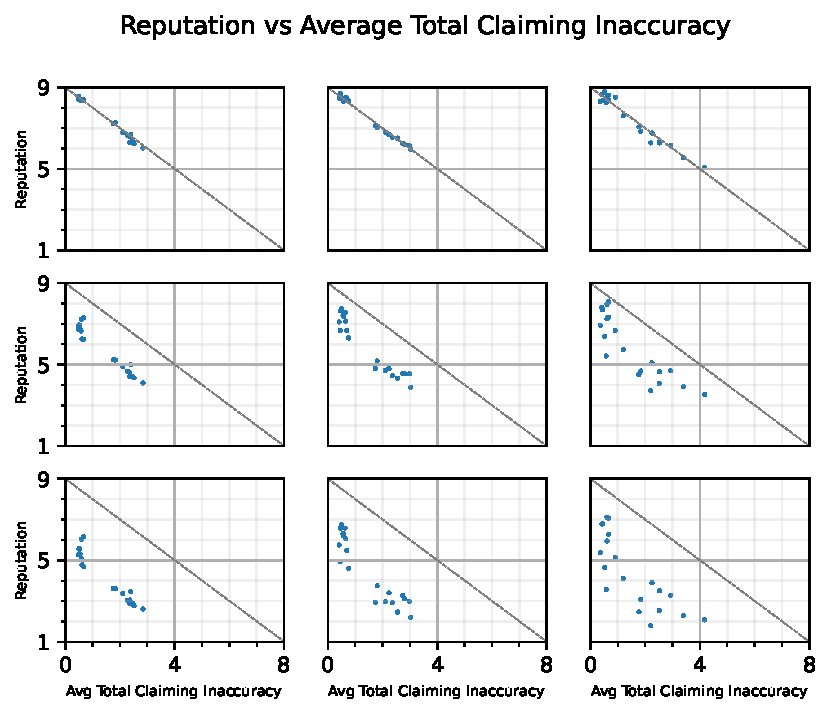
\includegraphics[width=0.75\linewidth]	{../results/a/AvgTotClaimInaccuracyAndReputationScatter_joined.pdf}
    \caption{
    Average Total Claiming Inaccuracy and reputation scatter diagram of experiment A: effect of aging.
    Aging increases toward the right column, while malicious raters increase toward the bottom row.
    }
    \label{fig:res_a_scatter}
  \end{center}
\end{figure}

\begin{figure}[tbp]
  \begin{center}
        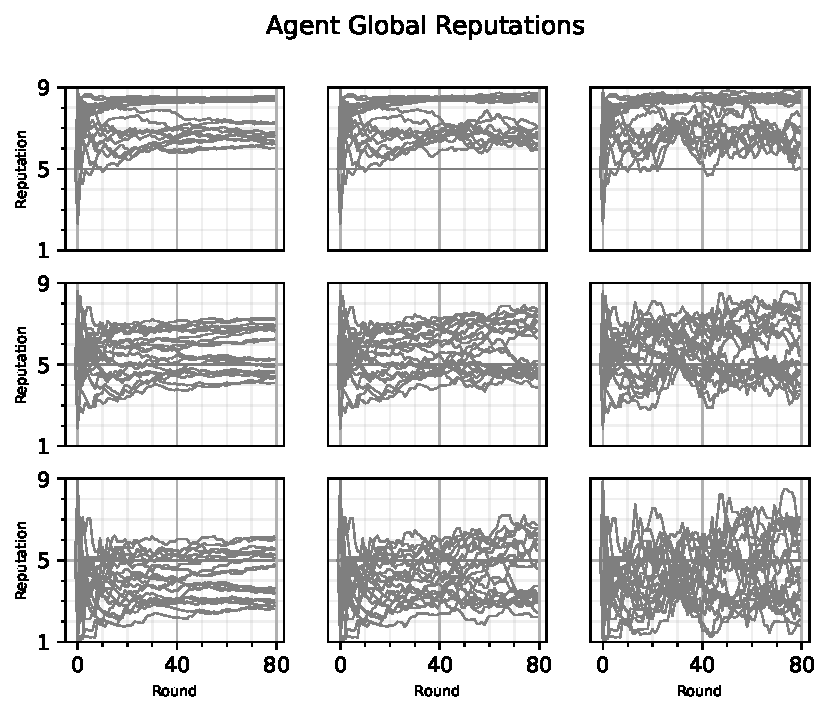
\includegraphics[width=0.75\linewidth]	{../results/a/ReputationsPerRounds_joined.pdf}
    \caption{
 	Progression of agent reputations per rounds in experiment A: effect of aging.
    Aging increases toward the right column, while malicious raters increase toward the bottom row.
    }
    \label{fig:res_a_reps}
  \end{center}
\end{figure}

\begin{figure}[tbp]
  \begin{center}
        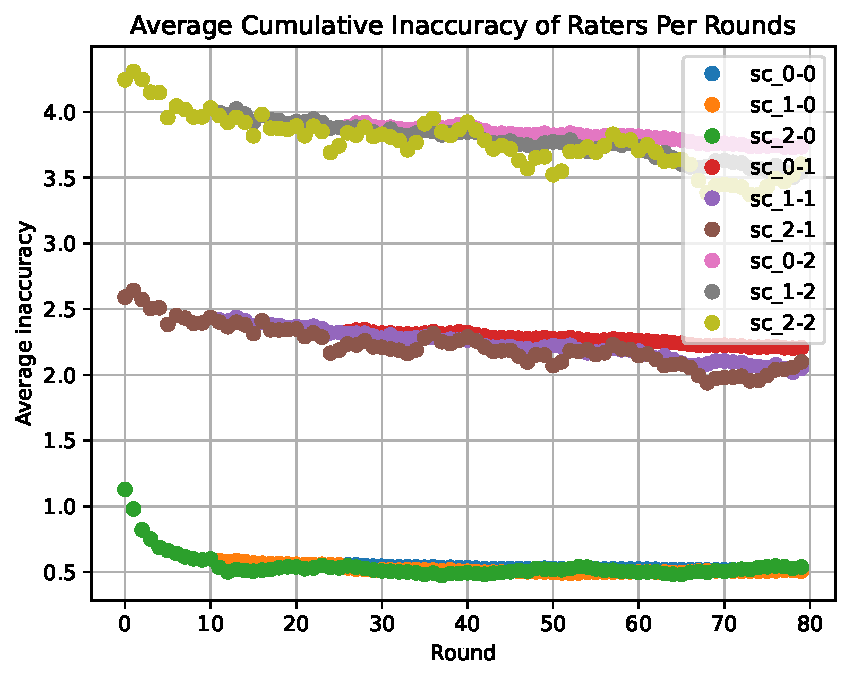
\includegraphics[width=0.75\linewidth]	{../results/a/AvgAccuracyPerRound.pdf}
    \caption{
    Averaged cumulative rater inaccuracy per rounds in experiment A: effect of aging.
    In the legend, first index increases with more aging, the second with more malicious agents.
    }
    \label{fig:res_a_rateinaccuracy}
  \end{center}
\end{figure}

\subsubsection{Experiment B: Malicious Raters}

Increasing the number of malicious raters results in a similar effect as observed in the previous experiment, only without the interference of aging.
Figure~\ref{fig:res_b_scatter} shows that malicious raters push the raputation of all claimers equally down.

Honest claimers are smeared towards their ideal reputation levels, as they form a sort of vertical line.
This means their inaccuracy was the same, still they received different reputations.
On the bottom row with all the raters malicious, the spread of honest claimer reputations is a little over 2 points.

Because malicious raters never claim, they do not get reputation adjustments and stay on the default of 5 for the whole simulation.
This means there is no way to filter their ratings, even with weights and a number of honest raters still in the system.

\begin{figure}[tbp]
  \begin{center}
        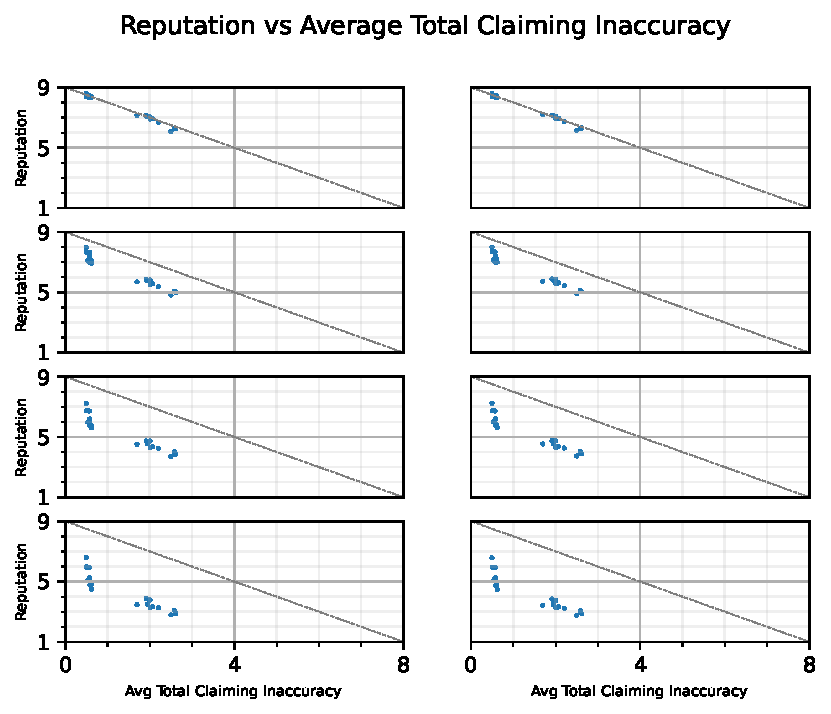
\includegraphics[width=0.75\linewidth]	{../results/b/AvgTotClaimInaccuracyAndReputationScatter_joined.pdf}
    \caption{
    Average Total Claiming Inaccuracy and reputation scatter diagram of experiment B: malicious raters.
    Malicious raters increase toward the bottom row.
    The left column is without any improvements, the right side is with weights enabled.
    }
    \label{fig:res_b_scatter}
  \end{center}
\end{figure}

\subsubsection{Experiment C: Dishonest Claimers}

C/I results are shown on figures \ref{fig:res_c_scatter} and \ref{fig:res_c_reps}.
Dishonest claimers are positioned above their exactly ideal reputation, but the difference is insignificant.
Good-intentioned raters are able to keep order even when all claimers are dishonest.
Figure~\ref{fig:res_c_reps} shows however, that it takes around 20-30 rounds for reputations to settle.
Both figures show no improvements on the left columns and weights on the right side.
There is no difference between the two versions.

\begin{figure}[tbp]
  \begin{center}
        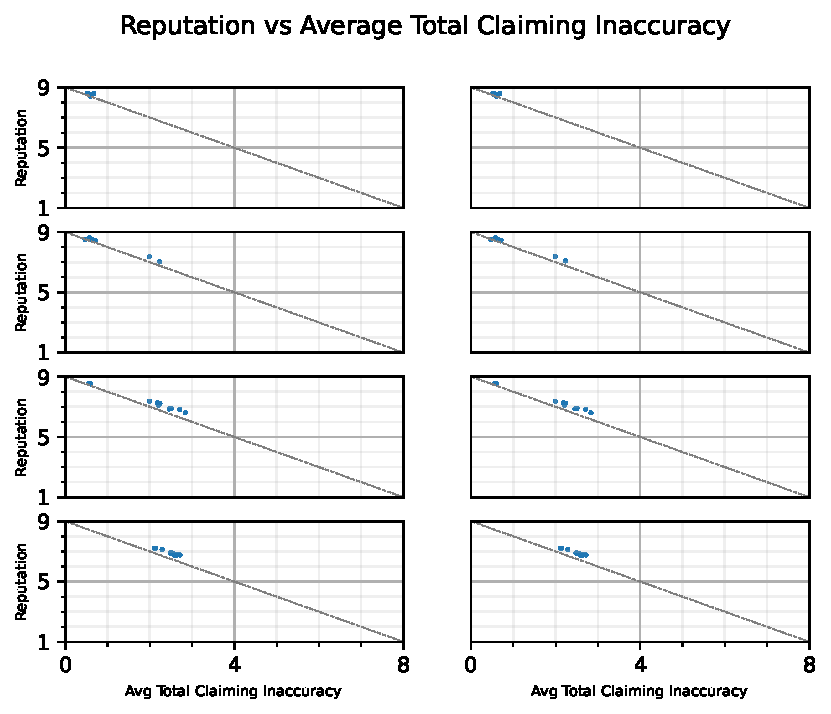
\includegraphics[width=0.75\linewidth]	{../results/c/AvgTotClaimInaccuracyAndReputationScatter_joined.pdf}
    \caption{
    Average Total Claiming Inaccuracy and reputation scatter diagram of experiment C/I: dishonest claimers.
    The number of dishonest claimers increases downwards.
    Left column: no improvements, right: weights enabled.
    }
    \label{fig:res_c_scatter}
  \end{center}
\end{figure}

\begin{figure}[tbp]
  \begin{center}
        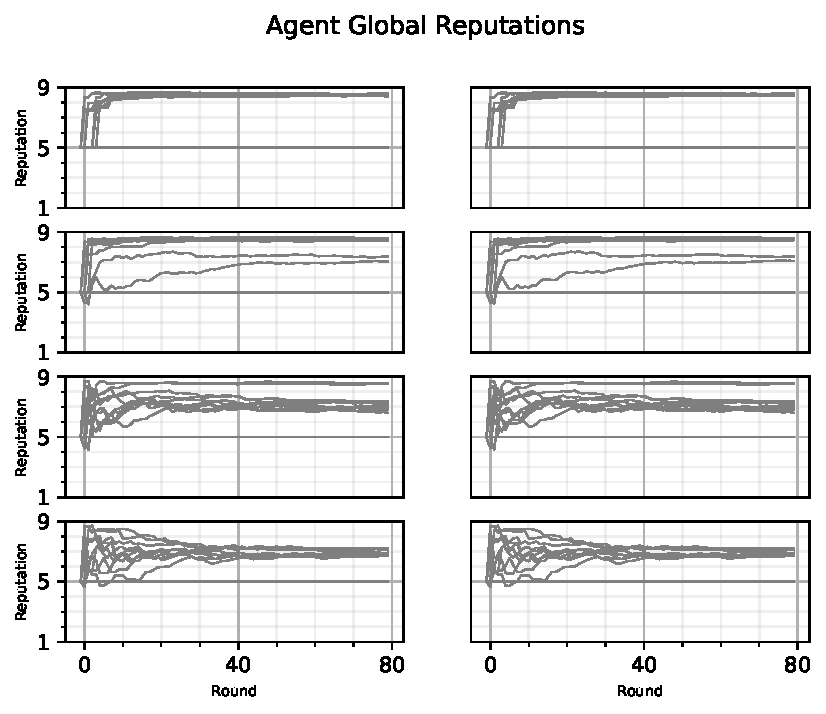
\includegraphics[width=0.75\linewidth]	{../results/c/ReputationsPerRounds_joined.pdf}
    \caption{
 	Progression of agent reputations per rounds in experiment C/I: dishonest claimers.
    The number of dishonest claimers increases downwards.
    Left column: no improvements, right: weights enabled.
    }
    \label{fig:res_c_reps}
  \end{center}
\end{figure}

Experiment C/II removes all raters that are not influencable, i.e. that are not \texttt{InfluencedHonestRater}.
It also tests the effect of higher \gls{ctai} for honest claimers and raters both.
As seen on figures ~\ref{fig:res_c2_scatter}, dishonest claimers are able to get an even better reputation by influencing raters with high author reviews.
In the right column, honest claimers have more inaccuracy, so they are more spread out horizontally on the total claiming inaccuracy axis.

Rater inaccuracy is also affected by the higher \gls{ctai}, shown on figure~\ref{fig:res_c2_rateinaccuracy}.
As expected, a higher \gls{ctai} makes reviews more inaccurate.

\begin{figure}[tbp]
  \begin{center}
        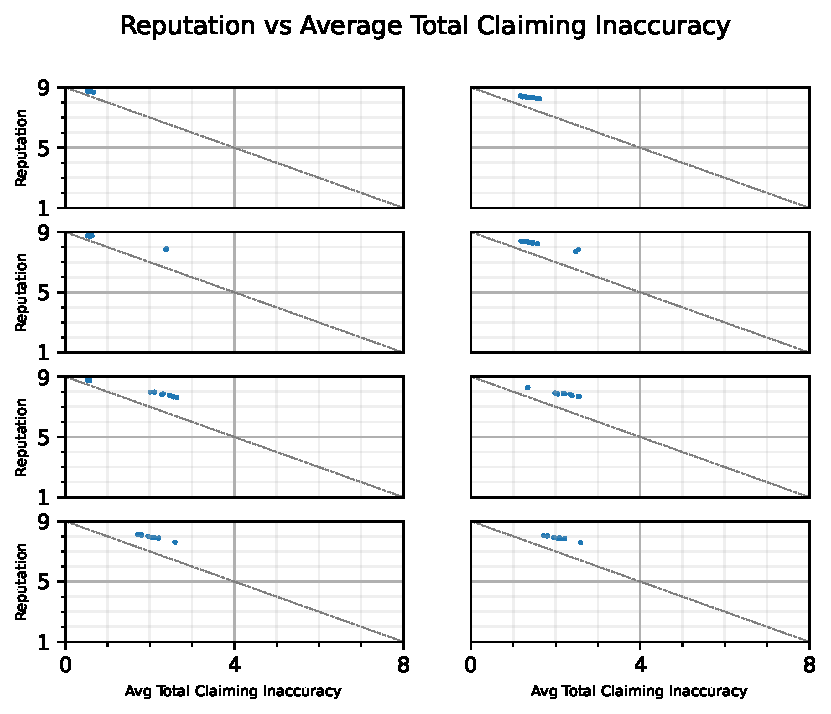
\includegraphics[width=0.75\linewidth]	{../results/c2/AvgTotClaimInaccuracyAndReputationScatter_joined.pdf}
    \caption{
    Average Total Claiming Inaccuracy and reputation scatter diagram of experiment C/II: dishonest claimers.
    The number of dishonest claimers increases downwards.
    Left column: honest raters and claimers have the default \gls{ctai}, right: \gls{ctai} is tripled for them.
    }
    \label{fig:res_c2_scatter}
  \end{center}
\end{figure}

\begin{figure}[tbp]
  \begin{center}
        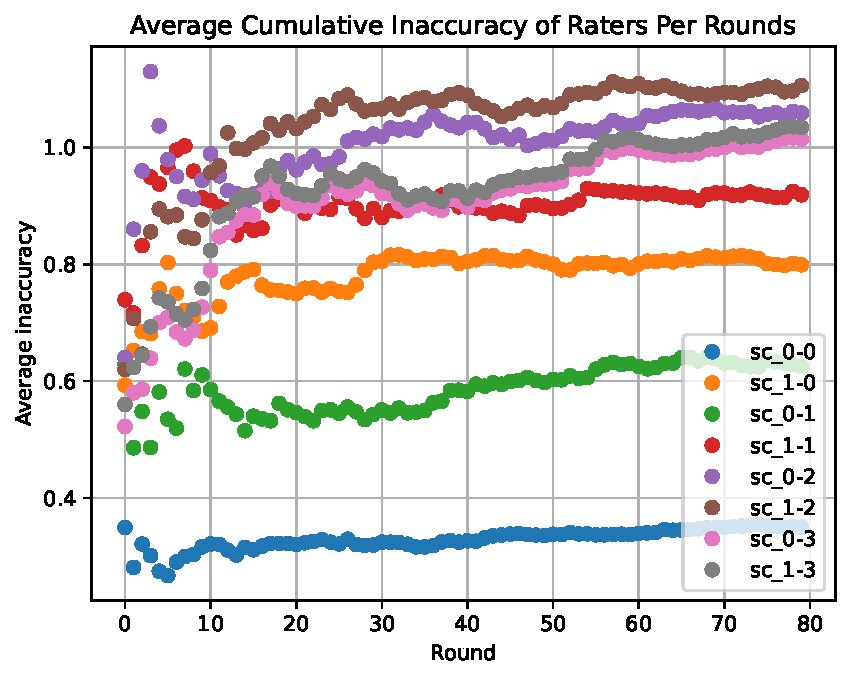
\includegraphics[width=0.75\linewidth]	{../results/c2/AvgAccuracyPerRound.pdf}
    \caption{
    Averaged cumulative rater inaccuracy per rounds in experiment C/II: dishonest claimers.
    In the legend, first index means lower \gls{ctai} if 0, higher if 1, applied only to hoenst raters and claimers.
    The second index increases along with the number of dishonest claimers.
    }
    \label{fig:res_c2_rateinaccuracy}
  \end{center}
\end{figure}

C/III simulates dishonest claimers that are dishonest increasingly often.
As observed on firugre~\ref{fig:res_c3_scatter}, dishonest claimers slide rightwards on the subfigures, meaning they make more and more dishonest claims.
With influencable raters, the dishonest claimers are able to acquire a better reputation.
In fact, the undeserved reputation gains get relatively larger as more and more dishonest claims are made.
However, if raters disregard the author's review (right, fig.~\ref{fig:res_c3_scatter}), reputation scores stay on the ideal line regardless of dishonest claims.

\begin{figure}[tbp]
  \begin{center}
        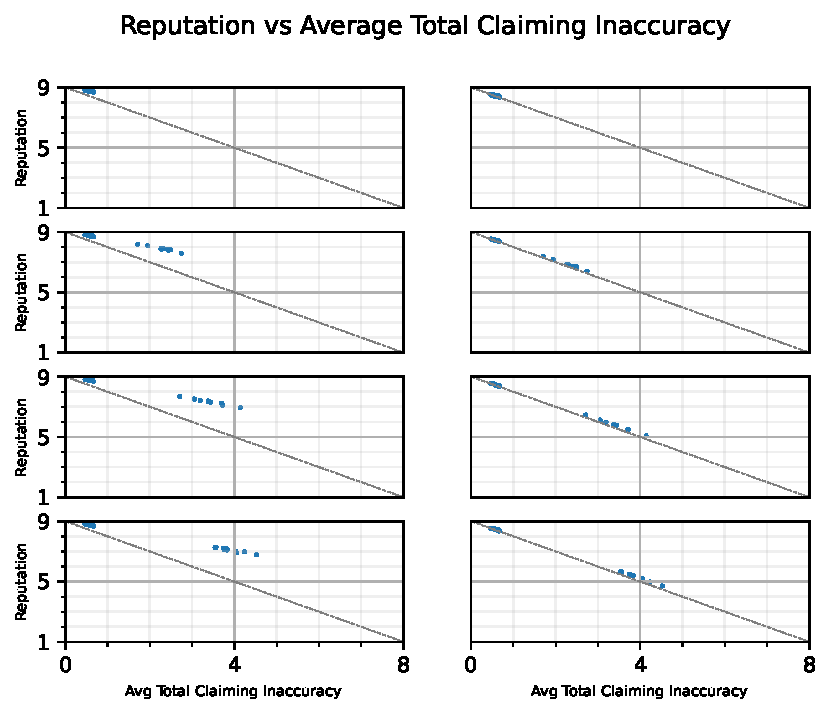
\includegraphics[width=0.75\linewidth]	{../results/c3/AvgTotClaimInaccuracyAndReputationScatter_joined.pdf}
    \caption{
    Average Total Claiming Inaccuracy and reputation scatter diagram of experiment C/III: dishonest claimers.
    Dishonest claimers make exaggerated maximum quality claims more often towards the bottom row.
    Left column: raters are influenced by author reviews, right: raters rely on their own experience only.
    }
    \label{fig:res_c3_scatter}
  \end{center}
\end{figure}

\subsubsection{Experiment D: Effect of Weights}

All agents are both raters and claimers in this experiment, because this is needed for them to have reputation adjusments.
D/I increases the number of dishonest agents.
Bad-intentioned raters are no longer malicious, instead they rate honest agents dogmatically with a lower score.
As expected, honest agent reputations are brought down, seen in fig.~\ref{fig:res_d_scatter}.
Using weights makes no difference here.

\begin{figure}[tbp]
  \begin{center}
        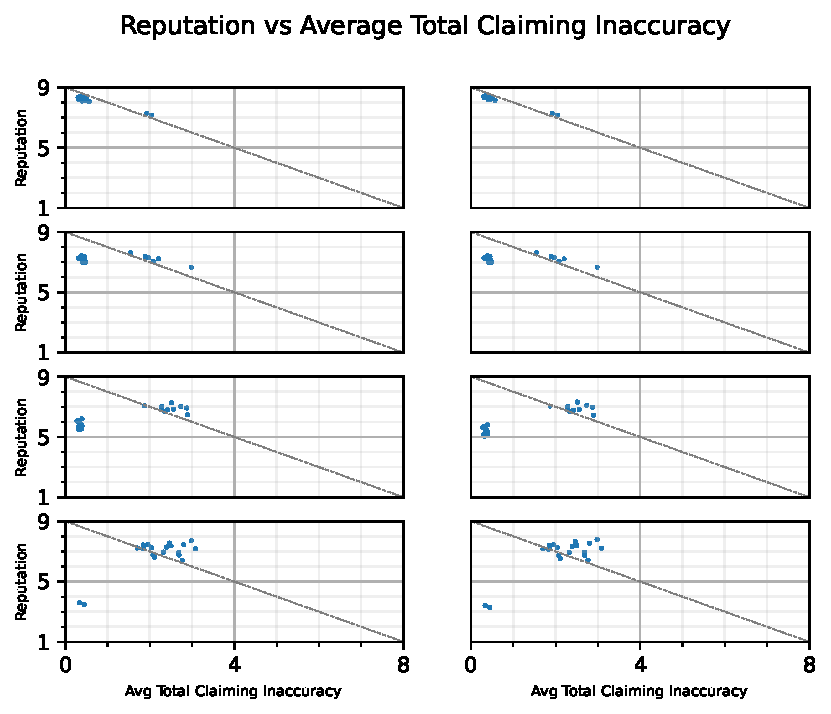
\includegraphics[width=0.75\linewidth]	{../results/d/AvgTotClaimInaccuracyAndReputationScatter_joined.pdf}
    \caption{
    Average Total Claiming Inaccuracy and reputation scatter diagram of experiment D/I: weights.
    The ratio of dishonest claimer-raters increases downwards.
    Both columns have aging with limit 30, right side also has weights.
    }
    \label{fig:res_d_scatter}
  \end{center}
\end{figure}

D/II makes agents dogmatic and divisive.
Honest agents give better ratings to good-reputation claimers and worse for bad-reputationed ones.
Dishonest agents claim dishonest every time.
Figure~\ref{fig:res_d2_scatter} shows that honest agents are able to recover their good reputation with the help of weights.
This is a relatively long process, taking 30-60 rounds (fig.~\ref{fig:res_d2_reps}).

\begin{figure}[tbp]
  \begin{center}
        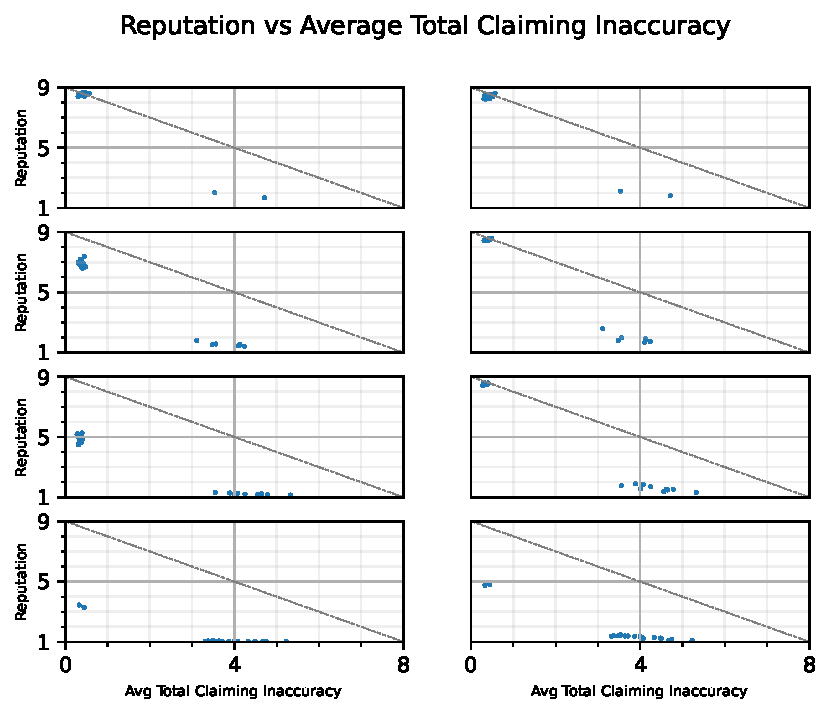
\includegraphics[width=0.75\linewidth]	{../results/d2/AvgTotClaimInaccuracyAndReputationScatter_joined.pdf}
    \caption{
    Average Total Claiming Inaccuracy and reputation scatter diagram of experiment D/II: weights.
    The ratio of dishonest claimer-raters increases downwards.
    Both columns have aging with limit 30, right side also has weights.
    Honest raters are dogmatic.
    }
    \label{fig:res_d2_scatter}
  \end{center}
\end{figure}

\begin{figure}[tbp]
  \begin{center}
        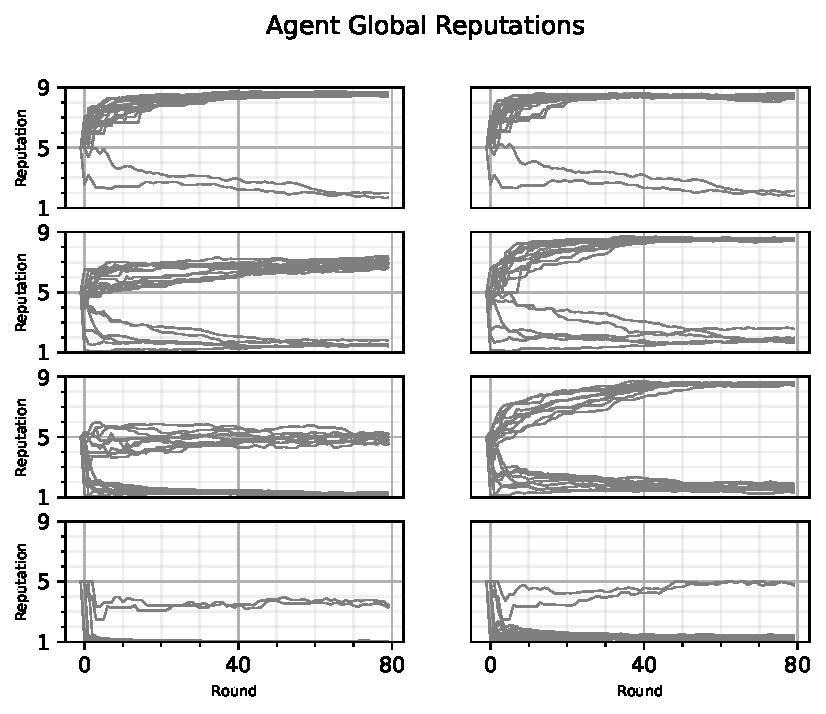
\includegraphics[width=0.75\linewidth]	{../results/d2/ReputationsPerRounds_joined.pdf}
    \caption{
 	Progression of agent reputations per rounds in experiment D/II: weights.
    The ratio of dishonest claimer-raters increases downwards.
    Both columns have aging with limit 30, right side also has weights.
    Honest agent reputations gradually recover with weights.
    }
    \label{fig:res_d2_reps}
  \end{center}
\end{figure}

In comparison, D/III results show that the same recovery of honest agent recovery no longer happens when the honest agents are not dogmatic.
On figure~\ref{fig:res_d3_scatter} all agents fall below the deserved ideal reputation line.
Weights pushes reputations closer to ideal, and all agents receive this effect.

\begin{figure}[tbp]
  \begin{center}
        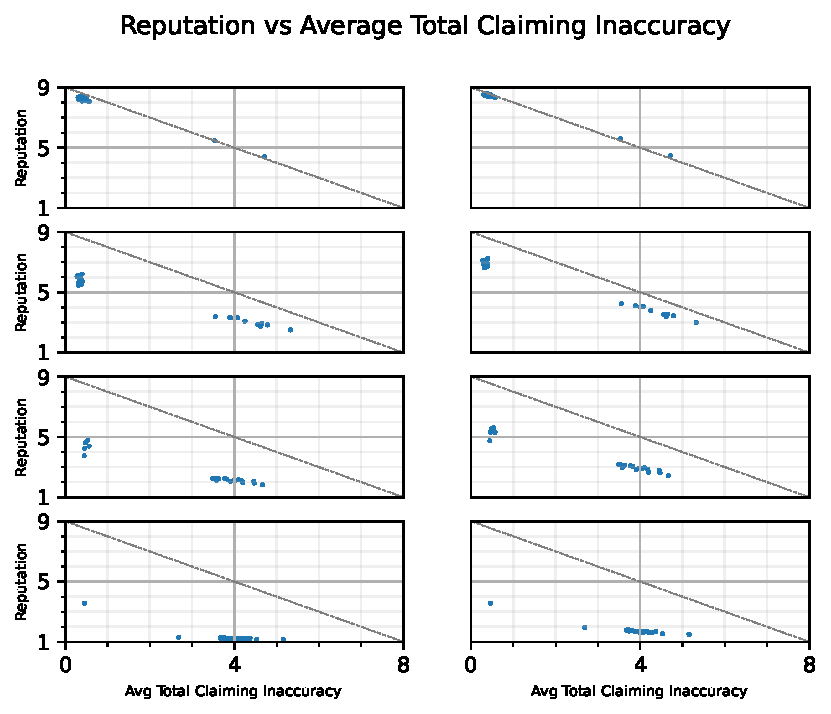
\includegraphics[width=0.75\linewidth]	{../results/d3/AvgTotClaimInaccuracyAndReputationScatter_joined.pdf}
    \caption{
    Average Total Claiming Inaccuracy and reputation scatter diagram of experiment D/III: weights.
    The ratio of dishonest claimer-raters increases downwards.
    Both columns have aging with limit 30, right side also has weights.
    Honest agents rate from their own experience.
    }
    \label{fig:res_d3_scatter}
  \end{center}
\end{figure}

\subsubsection{Experiment E: Measurement Accuracy}
Increasing the measuremend inaccuracy (\gls{ctai}) of agents is expected to have the effect of more inaccurate ratings, both author and regular.
This was partially shown in experiment C/II as well.
Here, inaccuracy is varied even more.

Figure~\ref{fig:res_e_rateinaccuracy} shows that rater inaccuracy generally increases with \gls{ctai}, as expected.
When 10 agents rate, the average inaccuracy is limited, while a single agent rates much more inaccurately.
Time makes sense, as the inaccuracies aaverage out for more agents.
Similar is observed in fig.~\ref{fig:res_e_reps}, where 10 completely inaccurate agents (bottom left) can set the reputations within 30 rounds, while a single agent with the same inaccuracy (bottom right) fails to arrive at the same reputations in 80 rounds.
Inaccurate raters can find out the reputation of agents accurately when they are in big numbers.

\begin{figure}[tbp]
  \begin{center}
        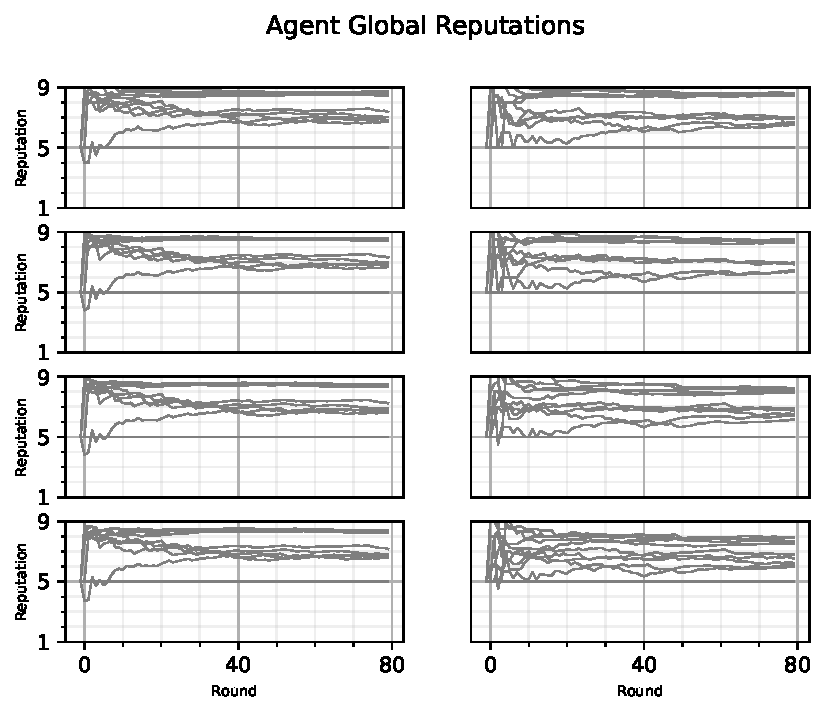
\includegraphics[width=0.75\linewidth]	{../results/e/ReputationsPerRounds_joined.pdf}
    \caption{
 	Progression of agent reputations per rounds in experiment E: measurement accuracy.
    \gls{ctai} increases downwards.
    Left: 10 raters, right: only 1 rater.
    }
    \label{fig:res_e_reps}
  \end{center}
\end{figure}

\begin{figure}[tbp]
  \begin{center}
        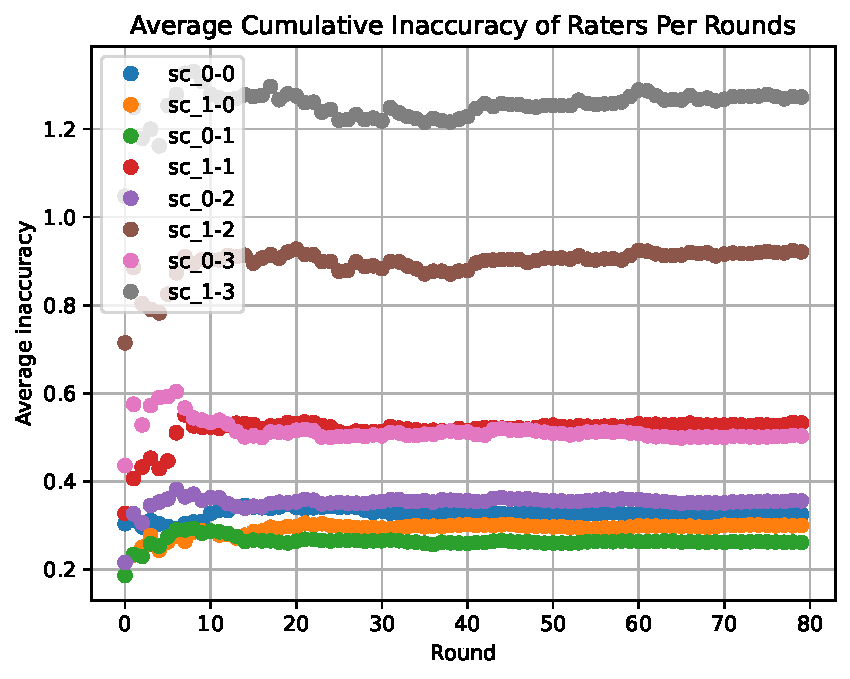
\includegraphics[width=0.75\linewidth]	{../results/e/AvgAccuracyPerRound.pdf}
    \caption{
    Averaged cumulative rater inaccuracy per rounds in experiment E: measurement accuracy.
    In the legend, first index means there are 10 raters if 0, only 1 rater if 1.
    The second index increases along with \gls{ctai}.
    More raters can balance measurement inaccuracy.
    }
    \label{fig:res_e_rateinaccuracy}
  \end{center}
\end{figure}

% --------------------------------------------------------------
\section{Discussion}\label{sec:discussion}
% --------------------------------------------------------------
%Discussion: Explain where, why, and to which extend you have or have not improved over related work. What does this mean for your initial problem question?


\subsubsection{Simulation Framework}
The created Pyrepsys framework fulfilled expectations, but not without remarks.
It turned out that the model has weaknesses with claiming and rating, some cases like environments with non-claimer raters are hard to handle.
A different reputation method and more elaborate agent behavior strategies could improve this.

Pyrepsys does not currently contain agent decision making for which claims agents interact with.
This is the basis of measuring agent success as metric, as stressed by the Alpha Testbed covered in chapter~\ref{chap:related_work}.
Such functinality would be possible to implement however.

Another weakness, which is also an advantage, is generality.
Not committing to specific domains or environments allows working in generics, but this also makes the model less specific.
When working within a concrete domain, a more niche evaluation framework can model the reputation environment better.

Pyrepsys is able to work without specifics of domains, and this is good when needed.
So far no universal and cross-domain evaluation frameworks gained widespread acceptance and use, even though researchers introduced multiple previously.
Simulating different kind of environments was possible and produced many of the expected results.
The simulator also manages to stay flexible and extendable, so it provides a viable alternative to other previous systems.


\subsubsection{Aging}
Aging was shown to make the reputation system's memory shorter.
While this was not particularly useful in tested experiments, it can have its uses.
When agent behaviors or qualities change, a reputation system should recognize this and adjust the agents reputation accordingly.
Examples for such change of behavior can be a different claiming method, or the agent gets more accurate or honest in claiming, or the other way around.
This is a realistic, since static behavior is rarely the case, even algorithmic agents can change abruptly with an update for example.
Aging's leniency to forget agent history makes a reputation system react faster to changes.

When selecting the aging time limit, the goal is to still produce more or less stable aggregations, so that reputation does not become erratic.
At the same time, the system should still allow changes over some timeframe.
Setting the aging limit needs to be tested for this in each different environment.

\subsubsection{Weights}
Weighting was shown to be helpful, but only under very specific configuration.
The weights implementation simply takes the agent's reputation and gives a proportional weight.
Since only claimers get reputation, purely rater agents never adjust their starting reputation, and so nor do they get weights.
When these same agents rate, their reviews will mostly be taken equally, because they all have default weights.
This was not the case with an agent population representing an algorithmic environment, where most raters are claimers as well.
Most other cases have this problem in the used model.

Either the weights method or the reputation calculation could change to resolve this.
If a reputation scheme can give reputation to raters who do not claim, the same simple weights can be used.
If the weight calculation is different, non-claiming raters should get weights assigned as well.

%a few dishonest can infiltrate, many dishonest can bring down honest reputations and get similar reps themselves
%note that dishonest agents do not cooperate here. if they were, they would probably be able to do better than anyone else


\subsubsection{Reputation Calculation}
The reputation method was seen to be lacking in cases where non-claiming raters exist.
This is most often the case, and allows malicious or dihonest behavior for raters.
To get this reputation method to work on rater side as well, the model would need some kind of second order rating, where reviews are rated as well.
Such systems exist already, for example online markets sometimes ask if a review was helpful or not.

%In cases where explicit claim quality measurement is possible, an automatic feedback mechanism could compare reviews the later measured with how the claim prediction turned out, and raters that predict well are rewarded

There are many different types of environments in which reputation systems are deployed.
Each has different circumstances, and it is difficult to find an approach that fits all.
Trust and reputation research is divided strongly into different domains, and this is a possible reason for that.


% CHAPTER ######################################################################
\chapter{Conclusion} \label{chap:conclusion}
% ##############################################################################
%Conclusion: Summarize main points; formulate key message.
%    Remind the readers what they have read and why it was significant. Don’t give new explanations, just the facts.
%    Repeat the most important result (number!) and what it means for the problem.
 
\lettrine{W}{e} successfully ...

% even with many different behavior models, reality can not be accurately represented
% in conclusion it can be said that accurately modeling reality within a reputation system is hard
% the difficulty rises even more if the aim is to stay generic
% without committing to a domain, all the domain-specific circumstances must remain abstracted, and since there are so many cases to cover for many domains, the end result can lose focus



% --------------------------------------------------------------
\section{Outlook}\label{sec:outlook}
% --------------------------------------------------------------

But we still need to ...






\begin{appendix}
\chapter{Scenario Configuration Options}\label{appendix:scenarios}
TODO comprehensive list of all scenario parameters

\chapter{Command Line Interface and Invocation}\label{appendix:cli_invocation}
TODO extensive CLI description

\chapter{Scenario Creator}\label{appendix:sc}
TODO SC desc

\end{appendix}


% Abbreviations
%	\printglossary[type=\acronymtype,title=Abbreviations]

% Glossaries 
\printglossary[type=acronym]       % print only acronyms

\printglossary

%\printglossaries                        % print all glossaries
%\printnoidxglossary[sort=word]
%\printnoidxglossaries


% ##############################################################################

%\nocite{*}   % use this to print all references

% print bibliography
% check if biblatex or legacy bibtex is used
\ifoptionbiblatex
    \printbibliography[heading=bibintoc]              % print BibLaTex bibliography
\else
    \addcontentsline{toc}{chapter}{Bibliography}
    \bibliographystyle{ieeetr}      % bibtex style
    \bibliography{references}       % bibtex library filename(s) WITHOUT extension
\fi


\end{document}


